\documentclass[11pt,a4paper]{article}

\usepackage[margin=26mm,headheight=15pt]{geometry}
\usepackage[T1]{fontenc}
\usepackage[utf8]{inputenc}
\usepackage{mathpazo}
\usepackage[scaled=0.92]{helvet}
\usepackage{microtype}
\usepackage{amsmath,amssymb,amsthm,mathtools}
\usepackage{mathrsfs}
\usepackage{bm}
\usepackage{booktabs,longtable,tabularx,array,multirow}
\usepackage{enumitem}
\usepackage{xcolor}
\usepackage{tikz}
\usetikzlibrary{arrows.meta,positioning,shapes.geometric}
\usepackage{graphicx}
\usepackage{fancyhdr}
\usepackage{natbib}
\usepackage{hyperref}
\usepackage[nameinlink,noabbrev]{cleveref}
\usepackage{listings}
\usepackage{seqsplit}
\usepackage{caption}
\usepackage{ragged2e}

\definecolor{inkblue}{RGB}{23,55,78}
\definecolor{rulegray}{RGB}{105,112,118}
\definecolor{softgray}{RGB}{244,246,247}
\hypersetup{
  colorlinks=true,
  linkcolor=inkblue,
  citecolor=inkblue,
  urlcolor=inkblue,
  pdftitle={On Boundaries of Evidence --- Boundary-State Calculus for Typed Observation, Admissible Transfer, and Falsifiable Persistence},
  pdfauthor={J. Tree},
  pdfsubject={A typed audit calculus for scientific transfers},
  pdfkeywords={Boundary-State Calculus, scientific transfer, evidence, admissibility, information loss, claim status}
}
\urlstyle{same}
\setlength{\parindent}{1.25em}
\setlength{\parskip}{0.15em}
\setcounter{secnumdepth}{3}
\setcounter{tocdepth}{2}
\setlist{nosep,leftmargin=1.7em}
\renewcommand{\arraystretch}{1.14}
\newcolumntype{Y}{>{\RaggedRight\arraybackslash}X}
\newcolumntype{L}[1]{>{\RaggedRight\arraybackslash}p{#1}}

\pagestyle{fancy}
\fancyhf{}
\fancyhead[L]{\small\textsc{On Boundaries of Evidence}}
\fancyhead[R]{\small\thepage}
\renewcommand{\headrulewidth}{0.35pt}

\theoremstyle{definition}
\newtheorem{definition}{Definition}[section]
\newtheorem{assumption}[definition]{Assumption}
\newtheorem{convention}[definition]{Convention}
\newtheorem{fixture}[definition]{Worked fixture}
\newtheorem{openproblem}[definition]{Open problem}
\theoremstyle{plain}
\newtheorem{lemma}[definition]{Lemma}
\newtheorem{proposition}[definition]{Proposition}
\newtheorem{theorem}[definition]{Theorem}
\newtheorem{corollary}[definition]{Corollary}
\newtheorem{conjecture}[definition]{Conjecture}
\theoremstyle{remark}
\newtheorem{heuristic}[definition]{Heuristic}
\newtheorem{analogy}[definition]{Analogy}
\newtheorem{numericalresult}[definition]{Numerical result}
\newtheorem{empiricalresult}[definition]{Empirical result}
\newtheorem{remark}[definition]{Remark}

\newcommand{\rightsquigarrowK}{\mathrel{\leadsto}}
\newcommand{\TV}{\mathrm{TV}}
\newcommand{\Prob}{\mathsf P}
\newcommand{\E}{\mathbb E}
\newcommand{\Obs}{\mathcal O}
\newcommand{\Cert}{\mathsf{Cert}}
\newcommand{\Def}{\mathsf{Def}}
\newcommand{\Stat}{\mathsf{Stat}}
\newcommand{\Prov}{\mathsf{Prov}}
\newcommand{\Id}{\mathrm{id}}
\newcommand{\supp}{\operatorname{supp}}
\newcommand{\Tr}{\operatorname{Tr}}
\newcommand{\Hom}{\operatorname{Hom}}
\newcommand{\coker}{\operatorname{coker}}
\newcommand{\rank}{\operatorname{rank}}
\newcommand{\kernel}{\operatorname{ker}}
\newcommand{\diam}{\operatorname{diam}}
\newcommand{\Lip}{\operatorname{Lip}}
\newcommand{\push}{_{\#}}
\newcommand{\blank}{\text{--}}

\title{\vspace{-1.3cm}\textbf{On Boundaries of Evidence}\\[0.3em]
\Large--- Boundary-State Calculus for Typed Observation,\\
Admissible Transfer, and Falsifiable Persistence}
\author{J. Tree\\[-0.15em]\small Independent researcher}
\date{24 July 2026}

\begin{document}
\maketitle
\vspace{-2.2em}

\begin{abstract}
Boundary-State Calculus (BSC) is developed here as a typed audit calculus for
finite open systems.  Its purpose is not to supply a new ontology, but to decide
when a claim remains warranted after boundary observation, quotienting,
instrument change, transport, coarse-graining, dynamics, reconstruction,
composition, and perturbation.  We retain the authoritative BSC system objects
and make explicit their measurable repair.  We add a typed morphism record
containing state and observable transport, stochastic simulation, equation
residual, naturality defect, directed statistical deficiency, physical
completion, and a certificate.  Composition theorems show how defects and
deficiencies accumulate and when a persistence claim must be demoted.

The calculus incorporates boundary trace and Dirichlet-to-Neumann response,
operational quantum quotients, Blackwell--Le Cam comparison of experiments,
Koopman residuals and ordered learnability limits, sheaf descent, structured
cospan composition, non-invertible defects, and rigorous scale limits.  It
separates topological charge from physical charge by requiring an explicit
bridge derived from a gauge structure, action, current, anomaly, boundary
condition, or measurement protocol.  A five-axis claim ledger and a
proof-dependency graph prevent local success from promoting unrelated claims.
Eight exact fixtures expose both admissible transfers and hard obstructions,
including a deterministic regression receipt.  The resulting formalism treats
persistence as an operational organizing principle:
a persistent object is a recursively maintained finite boundary-state, and
persistent identity is operational equivalence maintained under repeated
admissible folds across declared scales.  This principle is defined and made
falsifiable; it is not asserted as a universal law.
\end{abstract}

\tableofcontents
\newpage

\section{Scope and non-claims}\label{sec:scope}

BSC concerns a finite open system only after ``finite,'' ``open,'' and
``system'' have been operationally fixed.  Finiteness may mean bounded spatial
domain, finite observation horizon, finite resources, or finite state
cardinality; these meanings are not interchangeable.  Openness means that a
declared interface permits exchange with an exterior, not that all exterior
degrees of freedom are known.

\begin{definition}[Audit calculus]\label{def:audit}
BSC is the collection of typed objects, admissibility conditions, residuals,
loss measures, dependency rules, and certificates used to assess a claim about
a finite open system under observation, representation, transfer, scale,
dynamics, reconstruction, composition, and perturbation.
\end{definition}

This definition is deliberately narrower than several interpretations that
have accumulated around boundary language.  BSC is not a fundamental ontology,
a unified field theory, a proof of holography or quantum gravity, a theory of
consciousness, or a license to identify systems by visual resemblance.  A
boundary may be geometric, causal, administrative, statistical, or
instrumental; the type must be stated.  The words ``topological,'' ``recursive,''
and ``quantum'' carry no evidential force without their mathematical objects
and physical bridges.

\begin{convention}[Local promotion]\label{conv:localpromotion}
Evidence promotes only the claim node tested and those descendants whose
declared dependencies are satisfied.  It does not promote the framework, a
neighboring claim, or an application by association.
\end{convention}

\begin{convention}[Source discipline]\label{conv:source}
An internal derivation, peer-reviewed result, preprint, numerical execution,
and analogy are distinct source states.  A citation supplies provenance; it
does not supply a missing map or proof.
\end{convention}

The cited core corpus contains both durable mathematics and explicit later
repairs.  The relevant lineage is recorded in the source set
\citep{BSCvol1,BSCvol2,BSCvol3,BSCsecond}.  This paper keeps the
durable core, records the repairs, and excludes civic or metaphysical material
from mathematical inference.  No empirical result is reported from the corpus.

\section{Nomenclature, types, and front ledger}\label{sec:nomenclature}

\subsection{Basic types}

Unless stated otherwise, measurable spaces are standard Borel.  A Markov
kernel \(K:X\rightsquigarrow Y\) assigns a probability measure
\(K(x,\cdot)\) on \(Y\) measurably in \(x\).  Kernel composition is
\[
 (L\odot K)(x,A)=\int_Y L(y,A)\,K(x,dy).
\]
A measurable map \(f:X\to Y\) is identified with its Dirac kernel
\(\delta_f\).  We write \(B_b(X)\) for the bounded Borel measurable
real- or complex-valued functions on \(X\).  Norms, metrics, and units are
declared locally; quantities of unlike units are never added merely by
choosing coefficients.

\begin{longtable}{L{0.18\textwidth}L{0.31\textwidth}L{0.42\textwidth}}
\caption{Core nomenclature and types.}\label{tab:types}\\
\toprule
Symbol & Type & Role\\
\midrule
\endfirsthead
\toprule
Symbol & Type & Role\\
\midrule
\endhead
\(\Omega_\ell\) & bounded domain or finite carrier & physical or abstract
interior at scale \(\ell\); its meaning and units are declared\\
\(\partial_\varepsilon\Omega_\ell\) & measurable subdomain, or
\(\partial\Omega_\ell\) with trace regularity & finite sensor layer; never
silently identified with an ideal boundary trace\\
\(X_\ell,U_\ell,Y_\ell,C_\ell\) & standard Borel spaces & raw states,
controls, outputs, and contexts/calibrations\\
\(\sim_\ell\) & measurable equivalence relation on \(X_\ell\) &
observational, gauge, or representational equivalence; quotient
\(\bar X_\ell=X_\ell/{\sim_\ell}\) used only when standard Borel\\
\(\mathcal F_{\ell,t}\) & increasing sigma-algebras & legal information
available immediately before time \(t\)'s outcome\\
\(K_{\ell,t}^{X},H_{\ell,t}^{X}\) &
\(X_\ell\times U_\ell\times C_\ell\rightsquigarrow X_\ell,Y_\ell\) &
raw dynamics and observation kernels before quotient descent\\
\(K_{\ell,t}^{\rm dyn}\) &
\(\bar X_\ell\times U_\ell\times C_\ell\rightsquigarrow\bar X_\ell\) &
descended local dynamics after lumpability; superscript prevents collision with interscale
post-processing\\
\(H_{\ell,t}^{\rm obs}\) &
\(\bar X_\ell\times U_\ell\times C_\ell\rightsquigarrow Y_\ell\) &
descended instrument channel after quotient invariance\\
\(G_\ell\) & measurable loss/metric structure & comparison geometry with
units and domain stated\\
\(V_\ell\subseteq\bar X_\ell\) & measurable admissible region & viability,
safety, or model-validity domain\\
\(R_\ell\) & declared family of typed kernels/maps & inherited class of
scale, quotient, representation, or reconstruction maps; each use is
namespaced below\\
\(B_\ell\) & typed ledger & boundary flux, entropy, information,
calibration, degeneracy, and provenance entries\\
\(\Obs_\ell\) & vector space, \(C^*\)-algebra, or measurable function class &
declared accessible observables\\
\(\tau_\partial,\Lambda_\Omega,E_\partial,e_\partial\) & trace, response,
reconstruction relation, selected extension & distinct boundary operators;
their domains are not interchangeable\\
\(\mathfrak M_{\ell m}\) & typed morphism record & state/observable transfer,
loss, defects, completion, and certificate\\
\(\delta(\mathsf E,\mathsf F)\) & number in \([0,1]\) & directed deficiency:
ability of experiment \(\mathsf E\) to simulate \(\mathsf F\)\\
\(\Cert\) & finite structured record & assumptions, tolerances, hashes,
proof/execution receipts, sources, obligations, and status vector\\
\bottomrule
\end{longtable}

\subsection{Independent status axes}

\begin{definition}[Status vector]\label{def:status}
Every claim \(c\) carries
\[
\Stat(c)=
(s_{\rm math},s_{\rm emp},s_{\rm comp},s_{\rm src},s_{\rm tr}),
\]
with the following partially ordered axes:
\begin{align*}
s_{\rm math}&\in\{\text{ill-posed},\text{refuted},\text{conjectural},
\text{conditional},\text{proved}\},\\
s_{\rm emp}&\in\{\text{contradicted},\text{untested},\text{single study},
\text{replicated}\},\\
s_{\rm comp}&\in\{\text{failed},\text{unexecuted},\text{executed},
\text{exact receipt}\},\\
s_{\rm src}&\in\{\text{unchecked},\text{internal},\text{present proof},
\text{verified preprint},\text{verified publication}\},\\
s_{\rm tr}&\in\{\text{blocked},\text{local only},\text{bounded},
\text{certified}\}.
\end{align*}
Within each displayed set, entries are ordered from least to greatest support;
the resulting finite chains supply the meet used below.  The ordering is for
evidential propagation: it does not identify ``ill-posed'' with ``false'' or
``contradicted'' with ``untested.''  An axis may instead be marked not
applicable, in which case no edge may depend on it.  Coordinates are never
averaged.
\end{definition}

The ordering is evidential, not rhetorical.  For example, a proved theorem can
remain empirically untested; an exact execution can implement an ill-posed
physical encoding; a peer-reviewed source can be irrelevant to the asserted
bridge.

\begin{table}[htbp]
\centering
\scriptsize
\caption{Concise claim-status ledger at entry.  Every cell uses exactly one
status from \cref{def:status}, or N/A when that axis is inapplicable.}
\label{tab:frontledger}
\begin{tabularx}{\textwidth}{L{0.25\textwidth}L{0.12\textwidth}L{0.12\textwidth}L{0.13\textwidth}L{0.15\textwidth}Y}
\toprule
Claim & Math. & Empirical & Computation & Source & Transfer\\
\midrule
Kernel quotient descent & proved & N/A & N/A & present proof & certified\\
Morphism defect accumulation & proved & N/A & unexecuted & present proof &
bounded\\
Universal persistence principle & conjectural & untested & unexecuted &
internal & local only\\
Universal boundary reconstruction & refuted & N/A & unexecuted & present proof &
blocked\\
Specified Koopman impossibility classes & proved & N/A & N/A &
verified publication & local only\\
Winding determines electric charge & refuted & untested & unexecuted &
present proof & blocked\\
Klingman toroidal model yields QCD & ill-posed & untested & unexecuted &
verified publication & blocked\\
Fixtures F1--F7 & proved & N/A & unexecuted & present proof & local only\\
Fixture F8 universal claim & refuted & N/A & exact receipt & present proof &
local only\\
\bottomrule
\end{tabularx}
\end{table}

\subsection{Dependency graph}

A claim ledger is a directed acyclic graph \(D=(\mathcal C,E)\).  An edge
\(a\xrightarrow{J}b\) states that claim \(b\) depends on claim \(a\) on the
axis set \(J\subseteq\{\rm math,emp,comp,src,tr\}\).  Status propagates only
along named axes.

\begin{figure}[htbp]
\centering
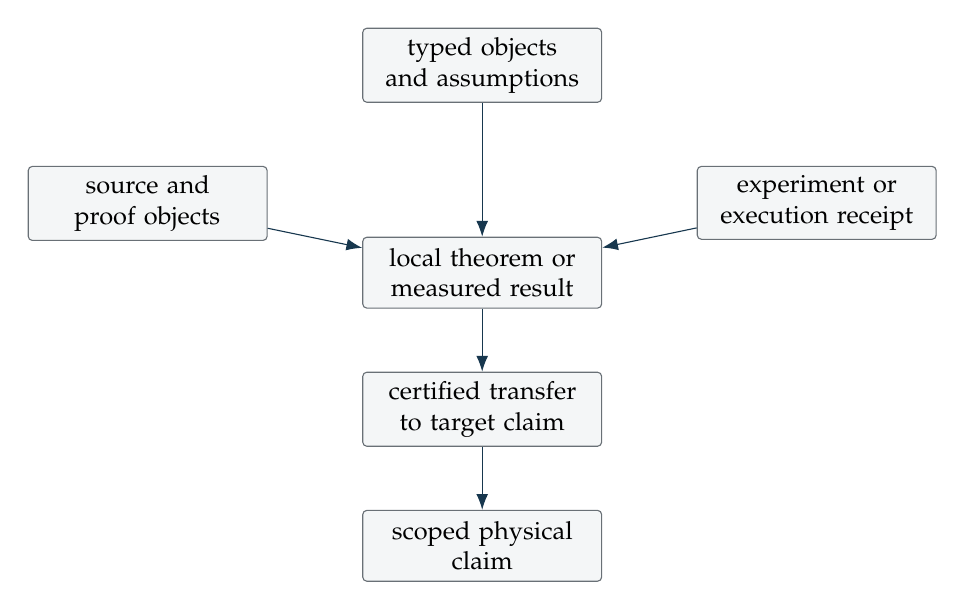
\begin{tikzpicture}[
  node distance=8mm and 12mm,
  box/.style={draw=rulegray,rounded corners=1.5pt,fill=softgray,
    align=center,text width=28mm,minimum height=9mm,font=\small},
  arr/.style={-{Latex[length=2mm]},draw=inkblue}
]
\node[box] (types) {typed objects\\and assumptions};
\node[box,below left=of types] (source) {source and\\proof objects};
\node[box,below right=of types] (tests) {experiment or\\execution receipt};
\node[box,below=17mm of types] (local) {local theorem or\\measured result};
\node[box,below=of local] (transfer) {certified transfer\\to target claim};
\node[box,below=of transfer] (physical) {scoped physical\\claim};
\draw[arr] (types) -- (local);
\draw[arr] (source) -- (local);
\draw[arr] (tests) -- (local);
\draw[arr] (local) -- (transfer);
\draw[arr] (transfer) -- (physical);
\end{tikzpicture}
\caption{Minimal dependency architecture.  Failure of an upstream requirement
demotes only descendants reached by the edge's declared status axes.}
\label{fig:dag}
\end{figure}

\begin{definition}[Demotion operator]\label{def:demotion}
For a claim \(b\), let \(\operatorname{Req}_j(b)\) be its immediate
predecessors on axis \(j\).  Its admissible status is bounded above by
\[
 s_j(b)\ \preceq\ \bigwedge_{a\in\operatorname{Req}_j(b)}s_j(a)
\]
unless \(b\) contains an independent certificate that discharges the
dependency.  New contradictory evidence applies the meet again.  Missing type
data makes the mathematical status ill-posed; missing execution makes only the
computational status unexecuted; a failed transfer makes only the deployment
status blocked unless it also supplies a mathematical counterexample.
\end{definition}

\section{Finite boundary-state systems}\label{sec:systems}

\subsection{Retained authoritative objects}

The original system object is retained exactly:
\begin{equation}\label{eq:originaltuple}
S_\ell(t)=
\left(
\Omega_\ell,\partial_\varepsilon\Omega_\ell,
X_\ell(t)/{\sim_\ell},U_\ell(t),Y_\ell(t),H_\ell,G_\ell,V_\ell,
R_\ell,K_\ell,B_\ell,\operatorname{rent}_\ell
\right).
\end{equation}
It records a finite domain, observed boundary layer, quotient state, controls,
outputs, observation, comparison geometry, viability, transformation class,
local dynamics, boundary ledger, and an admission penalty
\citep{BSCvol1}.  It is historically authoritative but under-typed: the context
used by \(H_\ell\) and the legal filtration are absent, \(R_\ell\) is
overloaded, and \(\operatorname{rent}_\ell\) has no fixed codomain.

The corpus then makes the following measurable repair, also retained exactly:
\begin{equation}\label{eq:currenttuple}
\widehat S_\ell=
\left(
\Omega_\ell,\partial_\varepsilon\Omega_\ell,X_\ell,{\sim_\ell},
U_\ell,Y_\ell,C_\ell,\mathcal F_\ell,K_\ell,H_\ell,G_\ell,V_\ell,
R_\ell,B_\ell
\right).
\end{equation}
Volume III explicitly works with \eqref{eq:currenttuple} while retaining the
application layers of the first object \citep{BSCvol2,BSCvol3}.  We therefore
take \(\widehat S_\ell\), not a newly invented tuple, as the current core.

\begin{definition}[Typed interpretation of \(\widehat S_\ell\)]
\(\Omega_\ell\) is a declared bounded domain or finite carrier;
\(\partial_\varepsilon\Omega_\ell\) is a measurable layer, with
\(\varepsilon\) carrying the domain's length or resolution unit.
\(X_\ell,U_\ell,Y_\ell,C_\ell\) are standard Borel spaces.  In particular,
\(C_\ell\) is a structured physical-configuration space containing the
instrument, observer or reference-frame state, controller, clock, and
calibration state needed by the experiment; omitting one of these factors is
a declared quotient, not a claim that the factor is nonphysical.
\(\sim_\ell\) is a measurable exact equivalence and
\(\bar X_\ell=X_\ell/{\sim_\ell}\) is required to be standard Borel whenever
ordinary quotient kernels are used.
\(\mathcal F_{\ell,t}\) is an increasing filtration.
\[
K_{\ell,t}^{X}:X_\ell\times U_\ell\times C_\ell\rightsquigarrow X_\ell,
\qquad
H_{\ell,t}^{X}:X_\ell\times U_\ell\times C_\ell\rightsquigarrow Y_\ell
\]
are the raw experiment kernels.  Write \(q_\ell:X_\ell\to\bar X_\ell\).
The observation kernel must be invariant,
\[
x\sim_\ell x'\Longrightarrow
H_{\ell,t}^{X}(\cdot\mid x,u,c)
=H_{\ell,t}^{X}(\cdot\mid x',u,c),
\]
and the dynamics must be lumpable,
\[
x\sim_\ell x'\Longrightarrow
(q_\ell)_\#K_{\ell,t}^{X}(\cdot\mid x,u,c)
=(q_\ell)_\#K_{\ell,t}^{X}(\cdot\mid x',u,c).
\]
Only then do quotient descent and the final sigma-algebra define the tuple's
operational kernels
\[
K_{\ell,t}^{\rm dyn}:\bar X_\ell\times U_\ell\times C_\ell
\rightsquigarrow\bar X_\ell,\qquad
H_{\ell,t}^{\rm obs}:\bar X_\ell\times U_\ell\times C_\ell
\rightsquigarrow Y_\ell .
\]
\(G_\ell\) is a declared metric, divergence, or measurable positive
semidefinite bilinear-form field; \(V_\ell\subseteq\bar X_\ell\) is measurable.
\(R_\ell\) is the inherited registry of typed scale, quotient,
representation, and reconstruction maps, never a single polymorphic arrow.
\(B_\ell\) is a schema of ledger entries, each with a value, unit, method,
uncertainty, time, and provenance.
Legal preparation and feedback are kernels
\[
\pi_{\ell,t}:(\mathsf H_{\ell,t},\mathcal F_{\ell,t})
\rightsquigarrow U_\ell\times C_\ell
\]
from the measurable observation history \(\mathsf H_{\ell,t}\); their
adaptedness means that \(\pi_{\ell,t}\) depends only on information in
\(\mathcal F_{\ell,t}\).  A state-Markov policy is separately denoted
\(\bar\pi_{\ell,t}:\bar X_\ell\rightsquigarrow U_\ell\times C_\ell\).
Such a policy, or a sufficient history augmentation of \(\bar X_\ell\), is
required before the joint kernels below induce a state-marginal fold.
\end{definition}

\begin{definition}[System certificate companion]\label{def:systemcert}
Without changing \eqref{eq:currenttuple}, associate
\[
\mathscr C_\ell=(D_\ell^{\rm rec},\Prov_\ell,\Cert_\ell),
\]
where \(D_\ell^{\rm rec}\) contains reconstruction relations and their
ambiguity classes; \(\Prov_\ell\) contains source identifiers, calibration
lineage, data and code hashes; and \(\Cert_\ell\) contains assumptions,
boundary conditions, tolerances, proof or execution objects, unresolved
obligations, and \(\Stat\).  The pair
\((\widehat S_\ell,\mathscr C_\ell)\) is an instantiated certified system, not
a replacement system tuple.
\end{definition}

\begin{definition}[Experiment bundle]\label{def:experimentbundle}
The retained experiment object is
\[
\mathcal E=(S,\mathcal T,\mathcal I,\mathcal M_0,\mathcal O,
\mathcal N,\mathcal L,\mathcal A,\mathcal D).
\]
Here \(S\) is \eqref{eq:currenttuple}; the repaired target is
\[
\mathcal T_{\rm src}=(Y,H,\tau,\mathcal F_t^{\rm legal}),
\]
where the source explicitly calls \(H\) the horizon but leaves \(\tau\)
undefined.  We set \(h:=H\), choose a declared finite sampling set
\(J_{t,h}\subset[t,t+h]\), and introduce a measurable target functional
\[
q:(Y^{J_{t,h}},\mathcal B(Y)^{\otimes J_{t,h}})\to Z_q .
\]
We then use the explicit repair
\[
\mathcal T^{\rm rep}=(Y,h,q,\mathcal F_t^{\rm legal}).
\]
The observation channel remains in \(S\) and is not duplicated in the target.
\(\mathcal I\) is the intervention class; \(\mathcal M_0\) a baseline;
\(\mathcal O\) candidate operators; \(\mathcal N\) matched nulls;
\(\mathcal L\) a scoring rule; \(\mathcal A\) an admission rule; and
\[
\mathcal D:\mathrm{Claims}\times\mathrm{Evidence}\to
\{\mathrm{admit},\mathrm{sandbox},\mathrm{watch},\mathrm{demote},
\mathrm{retire}\}.
\]
The name ``demotion map'' is retained, although its codomain also includes
admission.
\end{definition}

\subsection{Typed folds}

The original fold
\(\Pi_{V_m}^{G_m}\circ R_{\ell m}\circ H_\ell\circ K_\ell\)
mixes state dynamics, observation, inference, and state transport.  Its
architecture is useful but its displayed composite is not type-correct.

\begin{definition}[Lifted observation fold]\label{def:obsfold}
Put
\(\mathsf Z_\ell^{\rm sc}
=\bar X_\ell\times U_\ell\times C_\ell\).  Define
\begin{align*}
\widetilde K_\ell((x,u,c),d(x',u',c'))
 &=K_\ell^{\rm dyn}(dx'\mid x,u,c)\delta_u(du')\delta_c(dc'),\\
\widetilde H_\ell((x,u,c),d(y,c'))
 &=H_\ell^{\rm obs}(dy\mid x,u,c)\delta_c(dc').
\end{align*}
If \(R_{\ell m}^{Y}:Y_\ell\times C_\ell\rightsquigarrow\bar X_m\) is an
inference kernel and \(\Pi_{V_m}^{G_m}:\bar X_m\rightsquigarrow V_m\) a
declared measurable repair or projection kernel, then
\[
F_{\ell m}^{\rm obs}
=\Pi_{V_m}^{G_m}\odot R_{\ell m}^{Y}
\odot\widetilde H_\ell\odot\widetilde K_\ell
:\mathsf Z_\ell^{\rm sc}\rightsquigarrow V_m
\]
is a typed observation-to-state fold.  A direct state coarse-graining
\(R_{\ell m}^{X}:\bar X_\ell\rightsquigarrow\bar X_m\) defines a separate
route
\[
F_{\ell m}^{X}
=\Pi_{V_m}^{G_m}\odot R_{\ell m}^{X}\odot
\delta_{\pi_X}\odot\widetilde K_\ell,
\qquad
\pi_X:\mathsf Z_\ell^{\rm sc}\to\bar X_\ell .
\]
\end{definition}

Conflating these routes hides whether information was discarded by the
instrument, the inference, the quotient, or the scale map.

\section{Observation events, filtration, and leakage control}\label{sec:observation}

\begin{definition}[Observation atom]\label{def:atom}
The retained observation atom is
\[
a_t=(\ell,t,\Omega,\partial_\varepsilon\Omega,x_t,u_t,c_t,
H_t,y_t,\Sigma_{y,t},\mathcal F_t).
\]
It is legal for prediction horizon \(h>0\) when \(x_t\in\bar X_\ell\),
\(y_t\in Y_\ell\), and \(H_t=H_{\ell,t}^{\rm obs}\).  When
\(Y_\ell\subseteq\mathbb R^d\), \(\Sigma_{y,t}\in\mathbb R^{d\times d}\) is
positive semidefinite and has declared output units squared; for a general
output space it is replaced by a typed uncertainty object.
Every statistic used to predict \(Y_{t+h}\) is
\(\mathcal F_t\)-measurable.
\end{definition}

\begin{definition}[Boundary event]\label{def:boundaryevent}
For \(r\in\partial\Omega\),
\[
e_t=(r,t,J_k(r,t),X_k(r,t),\nu(r),\tau(r))
\]
records a flux/current component \(J_k\), boundary field \(X_k\), outward
normal \(\nu\), and orientation or time label \(\tau\).  Their tensor types and
units must be fixed by the governing model before any conservation checksum is
formed.
\end{definition}

\begin{assumption}[Pre-outcome freeze]\label{ass:freeze}
For an outcome at time \(t\), the design, preprocessing graph, dictionary,
candidate operators, null library, thresholds, and seed policy are
\(\mathcal F_{t-}\)-measurable.  Holdout outcomes and post-outcome edits are not.
\end{assumption}

\begin{definition}[Leakage defect]\label{def:leakage}
Let \(Z\) denote the complete fitted artifact and \(Y^{\rm hold}\) the
held-out outcome.  A protocol has structural leakage if \(Z\) is not measurable
with respect to the declared pre-outcome sigma-algebra.  A probabilistic
diagnostic is
\[
\lambda_{\rm leak}=I(Z;Y^{\rm hold}\mid\mathcal F_{t-}),
\]
when the conditional mutual information exists.  The diagnostic being zero
does not prove correct measurability; positive value refutes isolation.
\end{definition}

The earlier corpus condition that two sigma-algebras have empty intersection
is impossible because both contain the empty set and sample space.  The repair
is conditional isolation plus a logged access history.  If
\cref{ass:freeze} fails, computational or empirical promotion based on that
holdout is demoted regardless of predictive score.

\begin{proposition}[Predictable sequential admission]\label{prop:sequential}
Let \(A_t\) be false-admission events and let \(\alpha_t\) be
\(\mathcal F_{t-1}\)-measurable.  If
\(\Prob(A_t\mid\mathcal F_{t-1})\le\alpha_t\) almost surely and
\(\sum_t\alpha_t\le\alpha\), then
\(\Prob(\bigcup_tA_t)\le\alpha\).
\end{proposition}
\begin{proof}
Taking expectations gives \(\Prob(A_t)\le\E\alpha_t\).  The union bound and
Tonelli's theorem give
\(\Prob(\bigcup_tA_t)\le\sum_t\E\alpha_t
\le\E\sum_t\alpha_t\le\alpha\).
\end{proof}

This result does not validate the null model, exchangeability, or the physical
meaning of the score.  Those are separate dependencies.

\section{Boundary trace, response, and reconstruction}\label{sec:boundary}

Let \(\Omega\subset\mathbb R^n\) be bounded with boundary regularity stated
locally.  The following three operations are distinct.

\begin{definition}[Trace and layer]\label{def:trace}
For a Banach function space \(\mathcal X(\Omega)\) admitting a continuous trace,
\[
\tau_\partial:\mathcal X(\Omega)\to\mathcal X_\partial(\partial\Omega).
\]
For finite sensor resolution,
\[
\partial_\varepsilon\Omega
=\{x\in\Omega:\operatorname{dist}(x,\partial\Omega)\le\varepsilon\},
\qquad
L_\varepsilon:\mathcal X(\Omega)\to\mathcal Y_\varepsilon
\]
is a separate measurement map.  No equality
\(L_\varepsilon=\tau_\partial\) is presumed.
\end{definition}

\begin{definition}[Boundary response]\label{def:dtn}
Let \(L_a u=0\) be a declared elliptic boundary-value problem, with coefficient
\(a\) in an admissible class.  Let \(\mathcal B_D\) and \(\mathcal B_N\) be
the declared Dirichlet and conormal-response spaces.  In the standard weak
uniformly elliptic setting on a bounded Lipschitz domain one may take
\(\mathcal B_D=H^{1/2}(\partial\Omega)\) and
\(\mathcal B_N=H^{-1/2}(\partial\Omega)\).  If the weak solution \(u_f\) is
well posed for every \(f\in\mathcal B_D\), the Dirichlet-to-Neumann map is
\[
\Lambda_{a,\Omega}:\mathcal B_D\to\mathcal B_N,\qquad
f\longmapsto
\partial_{\nu,a}u_f\big|_{\partial\Omega},
\]
where \(\partial_{\nu,a}\) is the model's conormal derivative.  Thus
\(\Lambda_{a,\Omega}\) maps imposed boundary data to measured response; it is
not the trace of an arbitrary interior state.
\end{definition}

\begin{definition}[Reconstruction relation]\label{def:reconstruction}
For a data class \(\mathcal D\) and admissible interior class \(\mathcal A\),
\[
E_\partial\subseteq\mathcal D\times(\mathcal A/{\approx})
\]
is a possibly set-valued reconstruction relation.  The equivalence
\(\approx\) contains every gauge or boundary-fixing diffeomorphism ambiguity
left invariant by the data.  Identifiability means that each data item in the
range has at most one equivalence class; stability is a separate bound
\[
d_{\mathcal A/\approx}(a_1,a_2)
\le\omega\!\left(d_{\mathcal D}(\Lambda_{a_1},\Lambda_{a_2})\right)
\]
on a stated subset, for a declared modulus \(\omega\).
\end{definition}

\begin{definition}[Selected extension]\label{def:selectedextension}
For a declared subset \(\mathcal D_0\subseteq\mathcal D\), a selected
extension is a measurable map
\[
e_\partial:\mathcal D_0\to\mathcal X(\Omega)
\]
whose graph, after passage to the ambiguity class, lies in
\(E_\partial\).  Existence and measurability are assumptions; linearity and
boundedness are additional assumptions, never consequences of the
relation.  Any quantity evaluated on \(e_\partial(d)\) must either be
invariant under \(\approx\) or record the representative-selection
dependence.
\end{definition}

Scoped isotropic uniqueness theorems are available in the dimensions and
regularity classes of the cited works
\citep{sylvesteruhlmann1987,astalapaivarinta2006}.  In the anisotropic
manifold class of \citet{lassasuhlmann2001}, recovery is modulo the specified
boundary-fixing geometric equivalence.  Stability is weaker and separately conditional
\citep{alessandrini1988}.  None of these results licenses the phrase
``the boundary determines the interior'' without the PDE, data class,
regularity, quotient, boundary conditions, and stability theorem.

\begin{proposition}[Trace-limited prediction]\label{prop:tracelimited}
Let \(F:\mathcal X(\Omega)\to Z\) be \(L_F\)-Lipschitz and let a selected
extension \(e_\partial L_\varepsilon x\) be defined.  Then
\[
\|F(x)-F(e_\partial L_\varepsilon x)\|_Z
\le L_F\|x-e_\partial L_\varepsilon x\|_{\mathcal X}.
\]
\end{proposition}
\begin{proof}
This is the defining Lipschitz inequality.  It is an upper bound, not an
identifiability theorem.
\end{proof}

If additive data noise \(\eta\) is passed through a bounded linear selected
extension,
\(\|e_\partial\eta\|\le\|e_\partial\|\,\|\eta\|\).  The operator norm supplies
an upper worst-case amplification, not a universal lower error bound.

\section{Observable algebras and operational quotients}\label{sec:quotients}

\subsection{Classical experiment quotients}

\begin{definition}[Exact observation equivalence]\label{def:obseq}
For legal contexts and controls,
\[
x\sim_Hx'
\quad\Longleftrightarrow\quad
H^{X}(\cdot\mid x,u,c)
=H^{X}(\cdot\mid x',u,c)
\quad\text{for all legal }(u,c).
\]
A query \(q:X\to Z\) descends when it is constant on these classes.
\end{definition}

\begin{theorem}[Kernel quotient descent]\label{thm:quotient}
Let \(q:X\to\bar X=X/{\sim}\) be a measurable quotient of standard Borel
spaces, with the final sigma-algebra, and let \(M:X\rightsquigarrow Y\) be a
kernel constant on equivalence classes such that every coordinate
\(M(\,\cdot\,,A)\) is \(q\)-measurable.
Then there is a unique kernel \(\bar M:\bar X\rightsquigarrow Y\) satisfying
\(M=\bar M\odot\delta_q\).
\end{theorem}
\begin{proof}
For \(A\) in a countable generator of \(\mathcal B(Y)\), define
\(\bar M([x],A)=M(x,A)\).  Constancy makes this well defined.  Quotient
measurability and a monotone-class argument extend it to every Borel \(A\);
countable additivity is inherited pointwise.  Surjectivity of \(q\) gives
uniqueness.
\end{proof}

If \(\bar X\) is not standard Borel or stabilizer information matters, an
ordinary quotient is inadequate; a measurable groupoid or invariant-algebra
description is required.

\begin{definition}[Confusability pseudometric]\label{def:confusable}
Given a probability metric \(d_P\),
\[
d_E(x,x')=\sup_{(u,c)\ {\rm legal}}
d_P\!\left(H^{\rm obs}(\cdot\mid x,u,c),
H^{\rm obs}(\cdot\mid x',u,c)\right).
\]
The set \(d_E(x,x')\le\varepsilon\) is an identified neighborhood or
confusability graph relation.  It is not generally transitive and therefore
does not generally define a quotient.
\end{definition}

\subsection{Quantum operational quotients}

Let \(\mathcal H\) be finite-dimensional for the present definition, and let
\(\mathcal A_{\rm acc}\subseteq\mathcal B(\mathcal H)\) be the declared
operator system of accessible effects.

\begin{definition}[Operational quantum equivalence]\label{def:qequiv}
For density operators \(\rho,\sigma\),
\[
\rho\sim_{\mathcal A_{\rm acc}}\sigma
\quad\Longleftrightarrow\quad
\sup_{\substack{0\le E\le I\\E\in\mathcal A_{\rm acc}}}
|\Tr E(\rho-\sigma)|=0 .
\]
This is exact operational equivalence: equality of accessible probabilities,
not equality of matrix representations.  The pseudometric
\[
d_{\mathcal A_{\rm acc}}(\rho,\sigma)
=\sup_{\substack{0\le E\le I\\E\in\mathcal A_{\rm acc}}}
|\Tr E(\rho-\sigma)|
\]
defines \(\varepsilon\)-confusability by
\(d_{\mathcal A_{\rm acc}}(\rho,\sigma)\le\varepsilon\).  For
\(\varepsilon>0\) confusability is generally nontransitive and is not called
an equivalence.
\end{definition}

A state channel \(\Phi:\mathcal T(\mathcal H_\ell)\to
\mathcal T(\mathcal H_m)\) travels with its Heisenberg pullback
\[
\Phi^\sharp:\mathcal B(\mathcal H_m)\to\mathcal B(\mathcal H_\ell),
\qquad
\Tr[\Phi(\rho)A]=\Tr[\rho\,\Phi^\sharp(A)].
\]
Quantum reference-frame changes may alter which subalgebras count as
subsystems or accessible observables \citep{carette2025,ahmad2022,
castroruiz2025}.  Discarding is therefore relative to a declared algebra and
factorization, not an observer-free deletion operation.

\begin{definition}[Transform--discard defect]\label{def:discarddefect}
Let \(\Phi:\mathcal T(\mathcal H_R\otimes\mathcal H_S)\to
\mathcal T(\mathcal H_{R'}\otimes\mathcal H_{S'})\) be a frame or description
channel.  Suppose a candidate reduced channel
\(\bar\Phi:\mathcal T(\mathcal H_S)\to\mathcal T(\mathcal H_{S'})\) is
declared.  On accessible effects \(\mathcal A_{S'}\),
\[
\eta_{\rm td}(\rho)=
\sup_{\substack{0\le A\le I\\A\in\mathcal A_{S'}}}
\left|\Tr A\,\Tr_{R'}\Phi(\rho)
-\Tr A\,\bar\Phi(\Tr_R\rho)\right|.
\]
Transform and discard commute operationally on a class \(\mathcal Q\) when a
single \(\bar\Phi\) makes
\[
\sup_{\rho\in\mathcal Q}\eta_{\rm td}(\rho)=0.
\]
\end{definition}

\begin{proposition}[Paired transport preserves probabilities]\label{prop:paired}
For every state \(\rho\) and target effect \(A\),
\(\Tr[\Phi(\rho)A]=\Tr[\rho\Phi^\sharp(A)]\).  Consequently a representation
change is operationally harmless only for probabilities tested with the
paired observable transport.
\end{proposition}
\begin{proof}
This is the definition of the Banach adjoint \(\Phi^\sharp\).
\end{proof}

\section{Admissible morphisms and composition}\label{sec:morphisms}

The inherited deterministic morphism
\[
\mu_{a\to b}=(R_{a\to b},R_Y,\varepsilon_R,\tau_R,q_{a\to b})
\]
paired state and output maps with an error field, an otherwise untyped
\(\tau_R\), and quotient compatibility \citep{BSCvol1}.  In particular,
\(\tau_R\) is not silently promoted here to a certificate.  The printed
two-step error rule in that source is repaired to the type-correct downstream
Lipschitz bound
\[
\varepsilon_{ac}\le \varepsilon_{bc}+L_{bc}\varepsilon_{ab}.
\]
The later budgeted record is retained exactly as
\[
\mu=(R_X,R_Y,R_U,R_C,\alpha_H,\alpha_K,q_{ab},b_\mu),
\]
where \(q_{ab}\) records quotient compatibility and \(b_\mu\) a distortion
budget \citep{BSCvol2}.  Under explicit typing, \(R_X\) embeds in
\(T_{\ell m}\), \(R_Y\) in \(K_{\ell m}\), \(R_U,R_C\) in the completion,
\(\alpha_H,\alpha_K,b_\mu\) in the defect/tolerance fields, and \(q_{ab}\) in
the information-loss and admissibility fields.  The older \(R_{a\to b},R_Y\)
embed similarly; \(\varepsilon_R,\tau_R,q_{a\to b}\) are preserved in the
certificate until their types are discharged.  The following record extends
both; it does not replace the system object.

\begin{definition}[Typed BSC morphism]\label{def:morphism}
A morphism from certified system \(\ell\) to certified system \(m\) is
\begin{equation}\label{eq:morphism}
\mathfrak M_{\ell\to m}=
\left(
T_{\ell m},T_{\ell m}^{\sharp},K_{\ell m},R_{\ell m},
\Theta_{\ell m},\delta_{\ell m},C_{\ell m},\Cert_{\ell m}
\right),
\end{equation}
with a variant tag \(\mathsf v\in\{\mathrm{det},\mathrm{stoch},
\mathrm{quant},\mathrm{corr},\mathrm{defect}\}\).  For the stochastic variant:
\begin{enumerate}
\item \(T_{\ell m}:D_{\ell m}\rightsquigarrow\bar X_m\) is a Markov kernel on a
declared measurable domain \(D_{\ell m}\subseteq\bar X_\ell\).
\item
\[
T_{\ell m}^{\sharp}:B_b(\bar X_m)\to B_b(D_{\ell m}),\qquad
T_{\ell m}^{\sharp}g(x)=\int g(x')T_{\ell m}(x,dx')
\]
is positive and unital.  It need not be multiplicative.  In this bounded
stochastic variant, \(\Obs_i\subseteq B_b(\bar X_i)\), and the declared
observable families must satisfy
\[
T_{\ell m}^{\sharp}(\Obs_m)
\subseteq \Obs_\ell|_{D_{\ell m}} ;
\]
otherwise the state transfer does not transport the observables claimed.
Unbounded observables require a separately declared invariant integrability
domain.
\item \(K_{\ell m}:Y_\ell\rightsquigarrow Y_m\) is an observation
post-processing or simulation channel.
\item Given equation operators
\(\mathcal E_i:\mathsf{Dom}(\mathcal E_i)\to Z_i\) and an equation-space map
\(S_{\ell m}:Z_\ell\to Z_m\), the residual record \(R_{\ell m}\) contains
the target-equation residual, its Banach space, norm, units, evaluation class,
and bound.  In the deterministic variant,
\[
R_{\ell m}(x)=
\mathcal E_m(T_{\ell m}x)-S_{\ell m}\mathcal E_\ell(x)\in Z_m.
\]
For stochastic or nonlinear equations, the certificate must specify the
law-level weak residual; no canonical expectation is presumed.
\item Put
\(\mathsf Z_i^{\rm sc}=\bar X_i\times U_i\times C_i\).  The completion
\(C_{\ell m}\) contains control and context transports and a joint lift
\[
\widehat T_{\ell m}:
\widehat D_{\ell m}\rightsquigarrow\mathsf Z_m^{\rm sc},
\qquad
\widehat D_{\ell m}\subseteq\mathsf Z_\ell^{\rm sc},
\]
whose state marginal agrees with \(T_{\ell m}\) under the declared source
policy.  It also contains the physical carrier, controller, observer,
reference frame, instrument, clock map, resource interface, and boundary
conditions.
\item On the completed common domain,
\[
\Theta_{\ell m}
=\sup_{z\in\widehat D_{\ell m}} d_m\!\left(
H_m^{\rm obs}\odot\widehat T_{\ell m}(z),
K_{\ell m}\odot H_\ell^{\rm obs}(z)
\right)
\]
is a naturality or commuting-square defect in a declared probability metric.
\item For experiments
\(\mathsf E_i=\{P_{i,\theta}:\theta\in\Theta\}\),
\[
\delta_{\ell m}
=\delta(\mathsf E_\ell,\mathsf E_m)
=\inf_{K:Y_\ell\rightsquigarrow Y_m}
\sup_{\theta\in\Theta}
\|K P_{\ell,\theta}-P_{m,\theta}\|_{\TV}.
\]
The total-variation convention is
\(\|P-Q\|_{\TV}=\frac12\|p-q\|_1\) in the finite case.
For the particular implemented post-processor in the record, define
\[
e_{\ell m}(K_{\ell m})
=\sup_{\theta\in\Theta}
\|K_{\ell m}P_{\ell,\theta}-P_{m,\theta}\|_{\TV}
\ge\delta_{\ell m}.
\]
The certificate says whether this channel attains the infimum or is only a
declared near-minimizer.
\item \(\Cert_{\ell m}\) is the record specified in
\cref{def:systemcert}, augmented by variant, domains, tolerances, information
destroyed, residual and defect evaluations, implementation evidence, and
status vector.
\end{enumerate}
\end{definition}

A partial deterministic map uses the same record with explicit domain and
failure output.  A correspondence \(T\subseteq X_\ell\times X_m\) requires a
selection rule, multiplicity semantics, or probability kernel before
observable pullback is single-valued.  A quantum channel uses trace-class
states and its completely positive unital adjoint.  Defect and fusion variants
are treated in \cref{sec:open}.  These variants do not share a single
unqualified composition theorem.

\begin{definition}[Admissibility]\label{def:admissible}
\(\mathfrak M_{\ell m}\) is admissible for a declared claim only if its
certificate answers all of the following:
\begin{enumerate}
\item the domain, codomain, variant, regularity, units, and boundary conditions
of \(T_{\ell m}\);
\item the target observable class and reverse-direction transport
\(T_{\ell m}^{\sharp}\);
\item the equivalence classes or information distinctions destroyed;
\item the target equations, equation-space map, residual norm, and tolerance;
\item the observation and other diagrams tested, including nonzero defects;
\item the physical carrier, controller, clock, observer, reference frame, and
instrument that implement the transfer;
\item the assumptions, sources, proof objects, execution receipts, hashes,
unresolved obligations, and five-axis status.
\end{enumerate}
Failure to supply an item is a blocked transfer, not a small numerical error.
\end{definition}

\subsection{Composition in the stochastic variant}

\begin{assumption}[Compatible completions]\label{ass:completion}
For \(\mathfrak M_{\ell m}\) and \(\mathfrak M_{mn}\), the target interface,
clock, resource contract, boundary conditions, control/context law, and
carrier output of \(C_{\ell m}\) match the source requirements of \(C_{mn}\).
The composite completion is their specified fiber product over the shared
interface.  Moreover,
\(\widehat T_{\ell m}(z,\widehat D_{mn})=1\) for every
\(z\in\widehat D_{\ell m}\) in the composite domain.  Correlated failure
modes are retained.
\end{assumption}

\begin{definition}[Stochastic composite]\label{def:stochcomp}
Under \cref{ass:completion}, define
\[
T_{\ell n}=T_{mn}\odot T_{\ell m},\qquad
K_{\ell n}=K_{mn}\odot K_{\ell m},
\]
on the maximal measurable domain
\[
D_{\ell n}
=\{x\in D_{\ell m}:T_{\ell m}(x,D_{mn})=1\}.
\]
Then
\[
T_{\ell n}^{\sharp}
=T_{\ell m}^{\sharp}\circ T_{mn}^{\sharp}.
\]
On state--control--context space the compatible completion defines
\[
\widehat T_{\ell n}
=\widehat T_{mn}\odot\widehat T_{\ell m}.
\]
The certificate is the conjunction of assumptions and obligations, the union
of provenance DAGs, and the axiswise meet of statuses.  A new hash identifies
the composite record; it is not a new proof.
\end{definition}

\begin{theorem}[Observation-defect propagation]\label{thm:theta}
Let \(d_i=\|\cdot\|_{\TV}\), and let
\(\eta(K_{mn})\le1\) be the Dobrushin contraction coefficient of
\(K_{mn}\).  For compatible stochastic morphisms,
\[
\Theta_{\ell n}
\le \Theta_{mn}+\eta(K_{mn})\Theta_{\ell m}.
\]
For a Wasserstein metric, the same statement holds with the declared
Lipschitz coefficient of \(K_{mn}\), provided the required moments exist.
\end{theorem}
\begin{proof}
Apply the triangle inequality through the intermediate law
\(K_{mn}\odot H_m^{\rm obs}\odot\widehat T_{\ell m}\).  The first difference
is bounded by \(\Theta_{mn}\) after averaging over
\(\widehat T_{\ell m}\); the second contracts by \(\eta(K_{mn})\).  The
identity \(\widehat T_{\ell n}
=\widehat T_{mn}\odot\widehat T_{\ell m}\) supplies the other side of the
composite square.  Take the supremum.
\end{proof}

\begin{theorem}[Directed deficiency triangle]\label{thm:deftriangle}
Suppose all three experiments have the same parameter set \(\Theta\), or have
been pulled back to one by declared parameter maps.  Then
\[
\delta(\mathsf E_\ell,\mathsf E_n)
\le\delta(\mathsf E_\ell,\mathsf E_m)
  +\delta(\mathsf E_m,\mathsf E_n).
\]
\end{theorem}
\begin{proof}
Choose channels within \(\varepsilon\) of the two infima and compose them.
Total variation contracts under Markov kernels; the triangle inequality gives
the displayed bound plus \(2\varepsilon\).  Let \(\varepsilon\downarrow0\).
\end{proof}

\begin{theorem}[Deterministic equation-residual propagation]\label{thm:residual}
For deterministic state maps with
\(T_{\ell n}=T_{mn}T_{\ell m}\) and
\(S_{\ell n}=S_{mn}S_{\ell m}\), suppose \(S_{mn}:Z_m\to Z_n\) is bounded
linear, the equation domains are compatible, and
\(T_{\ell m}(D_{\ell m})\subseteq\mathsf{Dom}(R_{mn})\).  Then
\[
R_{\ell n}(x)
=R_{mn}(T_{\ell m}x)+S_{mn}R_{\ell m}(x).
\]
Consequently,
\[
\|R_{\ell n}\|_{\infty,D_{\ell m}}
\le \|R_{mn}\|_{\infty,T_{\ell m}(D_{\ell m})}
 +\|S_{mn}\|\,\|R_{\ell m}\|_{\infty,D_{\ell m}} .
\]
\end{theorem}
\begin{proof}
Add and subtract
\(S_{mn}\mathcal E_m(T_{\ell m}x)\) in
\(\mathcal E_n(T_{mn}T_{\ell m}x)
-S_{mn}S_{\ell m}\mathcal E_\ell(x)\).
\end{proof}

The identity morphism has \(T=\delta_{\Id}\), \(T^\sharp=\Id\),
\(K=\delta_{\Id}\), zero residual and defects, zero deficiency, identity
completion, and a certificate containing the relevant system identities.
Kernel associativity, reverse pullback composition, and the two fiber-product
unit isomorphisms give the unit laws.  If completion compatibility fails, the
composite is undefined rather than high-error.

\section{Defects, residuals, deficiency, and information loss}\label{sec:defects}

Residual, naturality defect, statistical deficiency, quotient loss, and
viability failure live in different spaces.  They are recorded as a vector,
not collapsed into a mechanism score.

\begin{definition}[Loss vector]\label{def:lossvector}
For a morphism, let \(\mathcal R_{\ell m}\) be its typed residual-record
space, let \(\mathcal Q_{\ell m}^{\rm res}\) be a declared residual test class,
and let
\[
\mathsf{ev}_{\ell m}^{\rm res}:
\mathcal R_{\ell m}\times\mathcal Q_{\ell m}^{\rm res}
\to[0,\infty]
\]
be a declared measurable scalar evaluator with recorded units.  Let
\(\mathcal Q_{\ell m}^{\rm law}\) be a declared class of admissible input
probability laws.  Put
\[
\mathcal L_{\ell m}=
\left(
\mathfrak r_{\ell m},
\Theta_{\ell m},
\delta_{\ell m},
e_{\ell m}(K_{\ell m}),
\lambda_{\rm quot},
\alpha_{\rm exit}
\right),
\]
where
\[
\mathfrak r_{\ell m}
=\sup_{\zeta\in\mathcal Q_{\ell m}^{\rm res}}
\mathsf{ev}_{\ell m}^{\rm res}(R_{\ell m},\zeta),
\qquad
\lambda_{\rm quot}(q)
=\sup_{x\sim_\ell x'}d_q(q(x),q(x'))
\]
for a measurable target query \(q:X_\ell\to(Q_q,d_q)\), and
\(\alpha_{\rm exit}=\sup_{\mu\in\mathcal Q_{\ell m}^{\rm law}}
\Prob_\mu(\tau_{V_m}\le h)\).  Here \(\tau_{V_m}\) is the first exit time
from \(V_m\) under the declared target dynamics and adapted policy.  An
important deterministic specialization takes
\(\mathcal Q_{\ell m}^{\rm res}=D_{\ell m}^{\rm eval}\) and
\(\mathsf{ev}^{\rm res}(R,x)=\|R(x)\|_{Z_m}\).  A law-level stochastic
residual instead requires its own weak-form evaluator; it is not inserted into
the deterministic formula.  Each coordinate has its own tolerance and
propagation law.
\end{definition}

\begin{definition}[Blackwell order]\label{def:blackwell}
Experiment \(\mathsf E_\ell\) Blackwell-dominates \(\mathsf E_m\), written
\(\mathsf E_\ell\succeq_B\mathsf E_m\), when a Markov kernel \(K\) satisfies
\(K P_{\ell,\theta}=P_{m,\theta}\) for every \(\theta\).  Thus
\(\delta(\mathsf E_\ell,\mathsf E_m)=0\): data from \(\ell\) can simulate
data from \(m\).  The converse deficiency may be positive.
\end{definition}

This direction follows \citet{blackwell1953} and \citet{lecam1964}, while
noting that conventions in the literature vary.  Only when needed do we use
\[
\Delta(\mathsf E,\mathsf F)
=\max\{\delta(\mathsf E,\mathsf F),\delta(\mathsf F,\mathsf E)\}.
\]
The directed deficiency itself is not a distance.

\begin{proposition}[Decision-risk consequence]\label{prop:risk}
For a bounded loss \(0\le L\le M\), if
\(\delta(\mathsf E,\mathsf F)\le\varepsilon\), then, for every
\(\eta>0\), every decision rule for
\(\mathsf F\) has a randomized rule based on \(\mathsf E\) whose worst-case
risk exceeds it by at most \(M(\varepsilon+\eta)\) under the present
total-variation convention.  If the deficiency infimum is attained and equals
\(\varepsilon\), one may take \(\eta=0\).
\end{proposition}
\begin{proof}
Use a channel within \(\eta\) of the deficiency infimum and then apply the
target decision rule.  The expectation of a function in \([0,M]\) changes by
at most \(M\|P-Q\|_{\TV}\).
\end{proof}

\begin{definition}[Boundary sufficiency gates]\label{def:boundarygates}
For a target \(Y_{t+h}\), boundary data \(X_{\partial,t}\), observed interior
\(X_{\Omega,t}^{\rm obs}\), exterior \(X_{{\rm ext},t}\), and legal covariates
\(Z_t\), define
\[
G_\partial=I(Y_{t+h};X_{\partial,t}\mid Z_t),\qquad
S_{\rm ext}=I(Y_{t+h};X_{{\rm ext},t}\mid
X_{\partial,t},X_{\Omega,t}^{\rm obs},Z_t).
\]
All logarithms are base \(2\), so \(G_\partial,S_{\rm ext},g_0,s_0\) are in
bits.
A target-relative statistical boundary claim requires
\(G_\partial\ge g_0\) and \(S_{\rm ext}\le s_0\) separately.  A large gain
cannot compensate for an open exterior channel.
\end{definition}

These are predictive diagnostics, not Sobolev traces, response maps, causal
carrier proofs, or coefficient reconstruction theorems.

\section{Dynamics, recurrence, Koopman operators, and learnability}
\label{sec:koopman}

Let \(F:X\to X\) be measurable on a probability space
\((X,\mathcal B,\mu)\).  When \(F\) preserves \(\mu\), the Koopman operator on
\(L^2(\mu)\) is the isometry
\begin{equation}\label{eq:koopman}
[\mathcal K_Fg](x)=g(F(x)).
\end{equation}
It acts on observables, not on states \citep{koopman1931}.

\begin{definition}[Certified approximate mode]\label{def:koopmode}
For a declared observable space \(\mathcal G\subseteq L^2(\mu)\),
\(\phi\in\mathcal G\) normalized by \(\|\phi\|_{L^2(\mu)}=1\), and
\(\lambda\in\mathbb C\),
\[
\varepsilon_{\rm dyn}(\phi,\lambda)
=\|\mathcal K_F\phi-\lambda\phi\|_{L^2(\mu)}.
\]
A nonnormalized nonzero mode is assessed by the corresponding relative
residual, dividing by \(\|\phi\|_{L^2(\mu)}\); \(\phi=0\) is inadmissible.
A certificate also states the dictionary, data-access model, norm, sampling
law, finite time horizon, limiting order, perturbation class, stability bound,
and learnability or Solvability Complexity Index class.
\end{definition}

Small training error is not this residual unless the sampling theorem and
dictionary-to-operator bridge are proved.  A finite compression can generate
spectral pollution.  Residual DMD supplies a posteriori rejection and
convergent spectral procedures for specified information models
\citep{colbrooktownsend2024,colbrookayton2023}.  It does not certify arbitrary
learned modes.

\begin{definition}[Recurrence and persistence]\label{def:persistence}
Let \((Q,d_Q)\) be Polish, let \(p\ge1\), and let
\(q_i:\bar X_i\to Q\) be declared identity observables.  Assume all
pushforward laws below lie in \(\mathcal P_p(Q)\).  For each \(i\), a completed
admissible fold
\(F_i:\mathsf Z_i^{\rm sc}
=\bar X_i\times U_i\times C_i\rightsquigarrow\bar X_{i+1}\)
and a certified filtration-adapted state-Markov policy \(\bar\pi_i\) induce
the state-marginal kernel
\[
P_i(x,A)=\int_{U_i\times C_i}
F_i((x,u,c),A)\,\bar\pi_i(d(u,c)\mid x).
\]
History-dependent policies require history augmentation of \(\bar X_i\);
without that augmentation the displayed Markov kernel is not asserted.
Let \(\mathbf X_0\sim\mu\in\mathcal P(\bar X_0)\) and
\(\mathbf X_{i+1}\mid\mathbf X_i\sim
P_i(\mathbf X_i,\cdot)\).  Denote the induced path law by \(\Prob_\mu\), and
define
\[
\tau_V=\inf\{i\ge0:\mathbf X_i\notin V_i\},
\qquad \inf\varnothing=\infty .
\]
Endpoint recurrence of a law \(\mu\) after \(n\) folds is
\[
\operatorname{Rec}_{q,n}(\mu)
=W_{p,Q}\!\left((q_0)\push\mu,\,
(q_n)\push(\mu P_0\cdots P_{n-1})\right).
\]
Persistent identity through \(n\) folds requires, for every prefix
\(k\le n\),
\[
W_{p,Q}\!\left((q_0)\push\mu,\,
(q_k)\push(\mu P_0\cdots P_{k-1})\right)\le\varepsilon_k,
\qquad
\Prob_\mu(\tau_V\le k)\le\alpha_k^{\rm cum},
\]
where \(\alpha_k^{\rm cum}\) is a cumulative exit budget, and every fold's morphism
certificate remains admissible.  Persistence is therefore stronger than
return at the final horizon.
\end{definition}

This formalizes, as an organizing principle, the statement:
\emph{a persistent object is a recursively maintained finite boundary-state;
persistent identity is an operational equivalence maintained under repeated
admissible folds across declared scales}.  It remains a target-relative
definition and conjectural physical principle, not a universal law.

\begin{theorem}[Prefix error budget]\label{thm:persistencebudget}
Suppose the identity discrepancy satisfies
\(E_{i+1}\le L_iE_i+e_i\), where \(L_i\ge0\) and \(e_i\ge0\) have common units.
Then
\[
E_n\le
\left(\prod_{j=0}^{n-1}L_j\right)E_0+
\sum_{i=0}^{n-1}e_i\prod_{j=i+1}^{n-1}L_j.
\]
Persistence is invalid at the first prefix whose bound exceeds its declared
tolerance, even if later contraction brings the endpoint below tolerance.
\end{theorem}
\begin{proof}
Induction on \(n\).  The prefix condition follows from
\cref{def:persistence}.
\end{proof}

Directed deficiencies satisfy the separate additive bound of
\cref{thm:deftriangle}; viability failures satisfy
\[
\Prob(\tau_V\le n)
\le\sum_{i=0}^{n}\beta_i
\]
without independence whenever the per-step bounds
\(\Prob(\mathbf X_i\notin V_i)\le\beta_i\) hold.  Alternatively the cumulative budget
in \cref{def:persistence} is checked directly as
\(\Prob(\tau_V\le n)\le\alpha_n^{\rm cum}\).  These coordinates must not be folded into
\(E_n\).

\subsection{Learnability boundary}

The Solvability Complexity Index records how many nested limiting processes a
specified computational problem requires and whether error control is
available \citep{colbrookhansen2023}.  Recent Koopman results give matching
success and impossibility regimes: for broad declared classes, some spectral
tasks require ordered limits, and no universal single-limit learner can solve
the stated problems; stronger structure restores certified algorithms
\citep{colbrookmezic2026}.  These are task-class impossibility results, not
impossibility of all forecasting.

\begin{convention}[Koopman claim gate]
A recurrence claim based on a learned operator is blocked unless it identifies:
(i) discrete eigenvalue, continuous spectrum, pseudospectrum, or spectral
measure as the target; (ii) the observable dictionary and its density claim;
(iii) the full or sampled residual; (iv) perturbation stability; (v) horizon
and sampling law; (vi) the order of limits; and (vii) the applicable positive
or negative learnability theorem.
\end{convention}

\section{Scale transfer, coarse-graining, and ordered limits}
\label{sec:scale}

\begin{definition}[Scale-limit certificate]\label{def:scalecert}
A micro-to-macro claim must state the record
\[
\begin{gathered}
(\varepsilon,\ \text{limit order},\ \text{scaling},\ \text{topology},
\ \text{boundary conditions},\\
\text{time interval},\ \text{uniformity domain},\ \text{effective
parameters},\ \text{error},\ \text{excluded regimes}).
\end{gathered}
\]
If more than one parameter tends to a limit, the certificate records whether
the limit is joint, iterated, or path-dependent.
\end{definition}

\begin{theorem}[Periodic elliptic homogenization]\label{thm:periodichom}
Let \(\Omega\subset\mathbb R^d\) be bounded and Lipschitz,
\(Y=(0,1)^d\), and let
\(A:\mathbb R^d\to\mathbb R^{d\times d}\) be measurable, symmetric, and
\(Y\)-periodic, with
\[
\lambda|\xi|^2\le \xi^\top A(y)\xi\le\Lambda|\xi|^2
\quad\text{a.e. }y,\quad \xi\in\mathbb R^d,
\]
for fixed \(0<\lambda\le\Lambda<\infty\).  For fixed
\(f\in H^{-1}(\Omega)\), let \(u_\varepsilon\in H_0^1(\Omega)\) be the
unique weak solution of
\[
-\nabla\!\cdot\!\bigl(A(x/\varepsilon)\nabla u_\varepsilon\bigr)=f .
\]
For \(j=1,\ldots,d\), let
\(\chi_j\in H_{\rm per}^1(Y)/\mathbb R\) solve
\[
\int_Y A(y)(e_j+\nabla\chi_j)\cdot\nabla v\,dy=0
\quad\text{for all }v\in H_{\rm per}^1(Y)/\mathbb R,
\]
and define
\[
A_{\rm hom}e_j=|Y|^{-1}\int_Y A(y)(e_j+\nabla\chi_j)\,dy .
\]
As \(\varepsilon\downarrow0\), after \(A,\Omega,f\) are fixed,
\[
u_\varepsilon\rightharpoonup u_0\ \text{in }H_0^1(\Omega),\qquad
u_\varepsilon\to u_0\ \text{in }L^2(\Omega),
\]
and
\[
A(x/\varepsilon)\nabla u_\varepsilon
\rightharpoonup A_{\rm hom}\nabla u_0
\quad\text{in }L^2(\Omega;\mathbb R^d),
\]
where \(u_0\in H_0^1(\Omega)\) solves
\(-\nabla\cdot(A_{\rm hom}\nabla u_0)=f\).
\end{theorem}
\begin{proof}
Uniform ellipticity and Lax--Milgram give a uniform \(H_0^1\) bound.
Weak compactness and Rellich compactness supply subsequential weak
\(H_0^1\) and strong \(L^2\) limits.  Periodic corrector test functions in
the weak formulation identify every subsequential flux limit with
\(A_{\rm hom}\nabla u_0\); uniqueness of the effective weak solution removes
subsequence dependence.  This is the standard corrector argument under the
displayed hypotheses \citep{bensoussanlionspapanicolaou1978}.
\end{proof}

This stationary theorem has no time limit.  It supplies no quantitative rate
under the stated hypotheses and no uniformity over changing coefficient
classes, data, or domains.  Degenerate, nonlinear, random,
oscillating-boundary, and coupled time-dependent regimes are excluded.
Stochastic
homogenization similarly exposes stationarity, mixing, dimension, and
ellipticity assumptions \citep{gloriaotto2012,armstrongsmart2016}.  This is the
model for BSC scale claims: no universal rate is inherited from the word
``coarse-graining.''

\begin{definition}[Dynamical scale defect]\label{def:scaledyn}
Let \((\bar X_b,d_b)\) be Polish.  For a measurable state map
\(R_{ab}^X:\bar X_a\to\bar X_b\), source and target Markov kernels
\(P_a,P_b\), and an input law \(\mu\) such that both displayed laws lie in
\(\mathcal P_p(\bar X_b)\), define
\[
T^{\rm dyn}_{ab}(\mu)=
W_p\!\left((R_{ab}^X)\push(\mu P_a),
((R_{ab}^X)\push\mu)P_b\right).
\]
\end{definition}

\begin{proposition}[Iterated scale defect]\label{prop:scaleiterate}
Suppose \(P_a,P_b\) preserve the required \(p\)-moments,
\[
T^{\rm dyn}_{ab}(\mu P_a^j)\le\tau
\quad\text{for }j=0,\ldots,n-1,
\]
and \(P_b\) is \(L_b\)-Lipschitz in the Wasserstein distance induced by
\(d_b\) on every propagated target law.  Then
\[
W_p\!\left((R_{ab}^X)\push(\mu P_a^n),
((R_{ab}^X)\push\mu)P_b^n\right)
\le\tau\sum_{k=0}^{n-1}L_b^k.
\]
\end{proposition}
\begin{proof}
Insert the one-step commuting square at each time and iterate the
Wasserstein triangle and Lipschitz inequalities.
\end{proof}

Classical kinetic-to-fluid limits exhibit the necessary scope
\citep{bardosgolselevermore1993,golsesaintraymond2004}.  The 2025 hard-sphere
program of \citet{denghanima2025} is a preprint result for a specified
hard-sphere \(\to\) Boltzmann \(\to\) Euler/Navier--Stokes--Fourier chain on
specified tori and ordered regimes, together with the long-time hard-sphere
derivation in \citet{denghanima2024}.  It is not a derivation of all continuum
mechanics or a settlement of every reading of Hilbert's sixth problem.  BSC
uses it as a case in disciplined scope, not as a universal bridge.

\section{Local-to-global consistency and sheaf obstruction}\label{sec:sheaf}

Let \(\mathcal U\) be a base of contexts closed under the finite intersections
and relevant unions used below, or replace it by the topology generated by the
declared cover.  More generally, the same definitions may be made on a site
after its Grothendieck topology is specified.

\begin{definition}[Observation sheaf]\label{def:sheaf}
An observation sheaf \(\mathscr F\) assigns to every context
\(U\in\mathcal U\) a set, vector space, or probability model
\(\mathscr F(U)\), and to \(V\subseteq U\) a restriction
\(\rho^U_V:\mathscr F(U)\to\mathscr F(V)\), with identity and composition
laws.  Local sections \(s_i\in\mathscr F(U_i)\) are compatible when
\[
\rho^{U_i}_{U_i\cap U_j}s_i
=\rho^{U_j}_{U_i\cap U_j}s_j
\]
for every nonempty overlap.  The sheaf axiom states that compatible sections
have a unique global section \(s\in\mathscr F(\bigcup_iU_i)\) restricting to
them.
\end{definition}

The last statement is an axiom of a chosen sheaf, not a fact about every data
assignment.  In contextual models one instead asks whether a compatible family
or local relation admits a global section; failure is the obstruction
\citep{abramskybrandenburger2011}.

\begin{definition}[Consistency operators]\label{def:sheaflap}
For a finite cell complex with finite-dimensional inner-product stalks, let
\(C^0\) be vertex assignments, \(C^1\) edge discrepancy spaces, and
\(d^0:C^0\to C^1\) the signed consistency difference constructed from the
cellular sheaf's coface maps.  This cellular coface convention is covariant
along face incidence and must not be confused with the contravariant
restriction maps of the ordinary sheaf in \cref{def:sheaf}.  The sheaf
Laplacian is
\[
L_{\mathscr F}=(d^0)^*d^0.
\]
Then \(\kernel L_{\mathscr F}=\kernel d^0\) is the space of exactly consistent
global assignments.  For data \(s\in C^0\), \(\|d^0s\|\) is a declared
consistency residual.  Its scale depends on the chosen inner products.
\end{definition}

This construction follows the finite cellular hypotheses of
\citet{hansenghrist2019}; it is not a canonical scalar for arbitrary
heterogeneous data.  For torsor-valued or parity constraints, a cocycle class
in \(H^1\) may obstruct gluing, but cohomology is invoked only after the
coefficient system and differential have been constructed.  The corpus's
earlier ``scale cohomology'' lacked these objects and is here demoted to path or
naturality defect.

\begin{proposition}[Gluing gate]\label{prop:gluing}
For an actual sheaf \(\mathscr F\), pairwise compatible local sections glue
uniquely.  For a presheaf, relation-valued assignment, or noisy family, local
nonemptiness alone does not imply a global section.
\end{proposition}
\begin{proof}
The first statement is the sheaf axiom.  The second is witnessed by
\cref{fix:sheaf}.
\end{proof}

\section{Open-system and non-invertible composition}\label{sec:open}

\subsection{A concrete interface category}

Let \(\mathcal T\) be a set of port types, including units and direction, and
let \(\mathsf I_{\mathcal T}\) be the full subcategory of
\(\mathrm{Set}/\mathcal T\) on maps \(p:A\to\mathcal T\) with finite domain.
Thus it is the category of finite typed interfaces even when \(\mathcal T\)
itself is infinite.  Let
\(\mathsf C\) be a category of internal carriers with finite colimits, and let
\(L:\mathsf I_{\mathcal T}\to\mathsf C\) embed an interface as a free boundary
carrier.

\begin{definition}[BSC decoration datum]\label{def:decoration}
Fix one mode
\(\mathsf r\in\{\mathrm{det},\mathrm{stoch},\mathrm{nondet}\}\) and one
compatible time object \(\mathbb T\).  A BSC decoration datum is a lax
symmetric monoidal functor
\[
\mathcal D_{\mathsf r,\mathbb T}:
(\mathsf C,+,0)\longrightarrow(\mathrm{Set},\times,1)
\]
with laxator
\(\varphi_{N,M}:\mathcal D(N)\times\mathcal D(M)\to
\mathcal D(N+M)\) and unit \(\varphi_0:1\to\mathcal D(0)\).
An element of \(\mathcal D(N)\) is a record
\[
d_N=(\widehat S_N,\mathsf r,\mathbb T,\mathsf{Beh}_N,\Cert_N),
\]
where \(\mathsf{Beh}_N\) is respectively a map/flow, Markov kernel, or
trajectory relation with typed boundary ports.  The functorial action
\(\mathcal D(f)\) specifies how behavior and certificates are transported
along a carrier map \(f\).  Illegal unit, clock, boundary, or resource
identifications map to a distinguished absorbing failed decoration and are
blocked by admissibility.  Mixed modes or clocks require a separately
declared lax monoidal comparison functor; they are not composed by default.
\end{definition}

\begin{definition}[Typed open BSC system]\label{def:cospan}
A deterministic, stochastic, or nondeterministic open system of the fixed
mode and clock from \(A\) to \(B\) is an isomorphism class of structured
cospans
\[
L(A)\xrightarrow{i}N\xleftarrow{o}L(B)
\]
decorated by \(d_N\in\mathcal D_{\mathsf r,\mathbb T}(N)\).
\end{definition}

Given \(A\to N\leftarrow B\) and \(B\to M\leftarrow C\), form the pushout
\(P=N+_{L(B)}M\) in \(\mathsf C\), with coprojections
\(j_N:N\to P\), \(j_M:M\to P\).  The composite is
\[
L(A)\longrightarrow N+_{L(B)}M\longleftarrow L(C),
\]
with decoration
\[
d_P
=\mathcal D([j_N,j_M])
\bigl(\varphi_{N,M}(d_N,d_M)\bigr).
\]
The identity on \(A\) is
\(L(A)\xrightarrow{\Id}L(A)\xleftarrow{\Id}L(A)\), decorated by
\[
d_A^{\rm id}
=\mathcal D(0\to L(A))(\varphi_0(*)).
\]

\begin{theorem}[Interface category]\label{thm:cospancat}
If \(\mathsf C\) has chosen finite colimits, \(L\) is a left adjoint and
strong symmetric monoidal for finite coproducts, and
\(\mathcal D_{\mathsf r,\mathbb T}\) is the decoration datum of
\cref{def:decoration}, then the objects of \(\mathsf I_{\mathcal T}\) and
morphisms of
\cref{def:cospan} form a category, up to the standard isomorphism classes.
Disjoint union supplies a symmetric monoidal product when the decorating
semantics is monoidal.
\end{theorem}
\begin{proof}
Pushout associativity and the universal property give associativity up to
canonical isomorphism; passing to isomorphism classes makes composition
associative.  Naturality and the associativity and unit axioms of the
laxator give the same laws for \(d_P\).  Identity cospans and
\(\varphi_0\) give the unit laws.
\end{proof}

This is the needed categorical construction, not decorative vocabulary.  It
is a BSC hybrid: structured cospans carry behavior and certificate
decorations.  Decorated and structured cospans are distinct constructions,
with precise comparison hypotheses
\citep{fong2015,baezcourser2020,baezcourservasilakopoulou2022}.
Heterogeneous internal types remain in the
apex decoration; only declared ports are identified.  Stochastic behavior may
also be organized in a Markov category, where copying and discarding are
structural but disintegration is not automatically available
\citep{fritz2020}.
Accordingly, equality-gluing of stochastic ports is legal here only when the
chosen \(\mathcal D_{\rm stoch,\mathbb T}\) explicitly supplies that
composition; no conditional distribution or disintegration is inferred from
the cospan alone.

\subsection{Non-invertible transports and defects}

\begin{definition}[Fusion morphism]\label{def:fusion}
Let \((\mathscr D,\otimes,\mathbf1,\alpha,\lambda,\rho)\) be a
\(k\)-linear additive monoidal category with finite biproducts.  A finite
fusion record is a finite family of defect objects \(D_a\in\mathscr D\),
including \(D_{\mathbf1}\simeq\mathbf1\), nonnegative integers
\(N_{ab}^{\ c}\) of finite support, and specified isomorphisms
\[
D_a\otimes D_b\simeq
\bigoplus_c D_c^{\oplus N_{ab}^{\ c}},
\]
coherent with the associator and unit constraints; equivalently their two
triple-fusion composites agree under the pentagon.  If the defects act on a
physical system \(A\), the record additionally supplies a monoidal functor
\(\mathscr D\to\operatorname{End}(A)\) in the declared ambient bicategory.
Vector-space or lower-dimensional-TFT multiplicities require an explicitly
tensored higher category and are a separate variant, not an untyped
replacement for the integers above.
\end{definition}

A quotient morphism pulls observables back only to the quotient-invariant
subalgebra.  A stochastic channel is generally irreversible and is compared by
deficiency.  A correspondence needs selection semantics.  A fusion morphism
branches, and the absence of an inverse is structural, not a failed group
axiom.  Physical use requires construction of the QFT, defect category,
fusion, anomaly, and boundary conditions; schematic fusion does not validate a
duality \citep{gaiotto2015,choi2022,apruzzi2023}.
Symmetry-TFT constructions further organize non-invertible defect data in
specified field theories; they do not supply a generic duality certificate
\citep{kaidiohmorizheng2022}.

\section{Topological quantities and physical charge}\label{sec:topcharge}

\begin{definition}[Topological charge]\label{def:topcharge}
Let \(A\) be an abelian coefficient group.  For
\([\omega]\in H^k(M;A)\) and \([C]\in H_k(M;\mathbb Z)\), the Kronecker
evaluation is
\[
Q_{\rm top}=\langle[\omega],[C]\rangle\in A .
\]
It is invariant under the stated homology/cohomology equivalences.  In the
differential-form case, \(A=\mathbb R\), \(\omega\) is a closed \(k\)-form,
and the de Rham pairing is \(Q_{\rm top}=\int_C\omega\), with any
normalization stated separately.
\end{definition}

\begin{definition}[Physical charge bridge]\label{def:chargebridge}
A physical charge is
\[
q_{\rm phys}=\chi(Q_{\rm top}),
\]
where \(\chi:A\to Q_{\rm phys}\) is a typed map into a declared physical
quantity space with charge units, derived from at least one declared physical
structure: gauge representation and coupling, an action and Noether current, a
Gauss-law boundary flux, anomaly constraint, boundary condition, or calibrated
measurement protocol.  Its normalization and units are part of the
derivation.
\end{definition}

\begin{proposition}[Normalization underdetermination]\label{thm:nocharge}
Let the only supplied carrier data be a winding invariant
\(Q_{\rm top}\in\mathbb Z\).  These data do not identify a real-valued
physical-charge map: they are compatible with every normalization
\(\chi_c:\mathbb Z\to\mathbb R\), \(\chi_c(n)=cn\), \(c\in\mathbb R\).
\end{proposition}
\begin{proof}
For every real constant \(c\), \(\chi_c(n)=cn\) is a group homomorphism.
The supplied data select none of the continuum of normalizations, nor the
electric unit, sign convention, matter representation, or coupling to an
electromagnetic current.  A nonlinear or quotient-valued bridge introduces
still more choices.
\end{proof}

Winding can be a valid topological carrier while the physical promotion is
blocked.  Modern monopole--center-vortex work illustrates the full price of a
bridge: it specifies \(SU(N)\) gauge theory, compactification, 't Hooft flux,
fractional topological charge, semiclassical action and fugacity, vacuum
branches, anomaly constraints, and representation-sensitive string tensions
in a controlled regime \citep{tanizakiunsal2022,hayashitanizaki2024}.  The
adiabatic passage to strongly coupled undeformed \(\mathbb R^4\) remains
conjectural in that work; it does not provide hadron spectroscopy or validate
an unrelated toroidal model.

\section{Certificates, claim ledgers, and demotion}\label{sec:certificates}

\begin{definition}[Certificate schema]\label{def:certschema}
A certificate is a machine-readable and human-inspectable record
\[
\begin{aligned}
\Cert=(\,&\mathsf{id},\mathsf{claim},\mathsf{types},\mathsf{assumptions},
\mathsf{tolerances},\mathsf{sources},\\
&\mathsf{artifacts},\mathsf{hashes},\mathsf{proof},\mathsf{execution},
\mathsf{obligations},\Stat).
\end{aligned}
\]
The proof field names the proposition and proof object or says
``mathematical proof in text.''  The execution field records code, inputs,
environment, command, output, tolerances, and receipt, or says
``unexecuted.''  Hashes identify artifacts; they do not establish truth.
\end{definition}

\begin{definition}[Mechanical verification]\label{def:mechanical}
A claim is mechanically verified only when a declared trusted kernel accepts
a proof object for the encoded proposition in a pinned environment.  The
certificate records the kernel and prover version, theorem identifier,
definitions, imported axioms, dependency hashes, build command, and accepted
output.  Kernel acceptance proves the encoded statement relative to those
foundations; it does not prove that the encoding represents the intended
physical system.
\end{definition}

Lean supplies a small-kernel architecture and explicit proof objects
\citep{demouraullrich2021}; large formalizations show the value of modular
dependency control \citep{hales2017,commelintopaz2024}.  A blueprint or proof
DAG is not itself a proof.

\begin{definition}[Numerical and empirical status]\label{def:numemp}
A numerical claim requires actual execution with code, inputs, environment,
output, convergence and tolerance criteria, and hashes.  A model description
without execution is computationally unexecuted.  An empirical claim also
requires a sampling frame, instrument and calibration, protocol, exclusions,
uncertainty analysis, and data provenance.  Simulation agreement is not
structural equivalence.
\end{definition}

\subsection{Corpus inheritance and local demotion}

The complete supplied corpus was treated as evidence under
\cref{conv:source}.  Table~\ref{tab:inheritance} records the disposition of
material not already represented by the retained tuples and morphism lineage.
The words ``retained'' and ``demoted'' apply locally to the listed statement,
not to an entire volume.

\begingroup
\small
\begin{longtable}{L{0.18\textwidth}L{0.35\textwidth}L{0.37\textwidth}}
\caption{Inheritance from the supplied BSC corpus.}\label{tab:inheritance}\\
\toprule
Source & Retained mathematical content & Status boundary\\
\midrule
\endfirsthead
\toprule
Source & Retained mathematical content & Status boundary\\
\midrule
\endhead
Volume IV \citep{BSCvol4} &
Identical observation laws imply a no-estimator obstruction; Fisher
information additivity and data processing, rollout/cascade bounds,
contraction criteria, entropy bookkeeping, and
\(I_{\rm classical}\le I_{\rm quantum}\) remain scoped mathematical
templates.  A boundary Poynting checksum must use an absolute residual or an
interval enclosure. &
The proposed optical and computational predictions are unexecuted here.
Signed cancellation is not accepted as a conservation certificate.\\
Volumes V--VI \citep{BSCvol5,BSCvol6} &
Exact quotient descent, non-descent of noninvariant queries, and Blackwell
comparison are retained where their hypotheses match this paper. &
Composite human-grounding scores, scaffold claims, and empirical programs are
unexecuted and untested; humane intent is not a mathematical bridge.\\
Second Catalogue and Volume VII \citep{BSCsecond,BSCvol7} &
Explicit repair discipline, bounded claims, and dependency-aware research
questions inform the certificate grammar. &
Civic, historical, and long-future meditations are outside the mathematical
dependency graph and receive no physical promotion.\\
Arithmetic Recursive Folds \citep{tree2026arithmeticfolds} &
Finite sieve identities and the declared Mellin-transform backbone survive as
ordinary arithmetic analysis. &
Primitive-orbit language is an analogy unless an operator and trace formula
are constructed; no Riemann-hypothesis proof is inherited.\\
Certified Arithmetic Trace Reconstruction
\citep{tree2026tracereconstruction} &
The finite-matrix prime-comb obstruction and the locally finite
arithmetic-density construction are retained in their stated classes. &
The prime-local operator fold is conjectural; finite truncations do not
certify an infinite spectral correspondence.\\
Derived Witnessed Descent \citep{tree2026deriveddescent} &
Strict, derived, and observed-derived holonomy are separate gates; a locally
finite \(0\)-chain has a natural atomic Radon-measure realization; the stated
distributionally closed smooth counterterm class collapses. &
No derived or observed gate is promoted by satisfying only the strict gate.\\
Formal Verification supplement \citep{formalverification2026} &
The bounded-jet orthogonal-prime-block obstruction is retained only under its
explicit hypotheses and quantifiers. &
Mechanical runs described in the source are source-asserted, not replayed:
the generating scripts and accepted JSON/proof receipts were not supplied.
Their computational status is therefore unexecuted here.\\
\bottomrule
\end{longtable}
\endgroup

\subsection{Explicit demotion rules}

\begin{enumerate}
\item An undefined domain, codomain, unit, quotient, or boundary condition
demotes the mathematical axis to ill-posed.
\item A counterexample demotes the quantified mathematical claim to refuted;
a repaired restricted claim receives a new identifier.
\item A proof sketch with an open lemma is conditional or conjectural, not
proved.
\item Failure of a leakage gate invalidates promotion from the affected
evaluation.
\item A numerical result without a reproducible receipt is unexecuted; a failed
build is failed.
\item A verified preprint is not recorded as peer reviewed.
\item If an upstream dependency is demoted, descendants inherit the axiswise
meet under \cref{def:demotion}.
\item Exceeding any prefix persistence tolerance blocks persistence at that
horizon; later recovery does not erase the excursion.
\item A successful transfer outside its declared domain is local only; using it
in a new domain requires a new morphism certificate.
\item An analogy may motivate a test but cannot occupy a mechanism dependency
slot.
\end{enumerate}

\section{Proven formal consequences}\label{sec:consequences}

This section collects consequences established in the present paper.  Their
scope is exactly the hypotheses cited; no empirical coordinate is promoted.

\begin{theorem}[Admissible-chain bound]\label{thm:chain}
For a compatible chain of stochastic BSC morphisms
\(\mathfrak M_{0,1},\ldots,\mathfrak M_{n-1,n}\), let
\(\eta_i\) be the observation-channel contraction of the \(i\)-th
post-processor and \(\theta_i=\Theta_{i,i+1}\).  Then
\[
\Theta_{0n}\le
\theta_{n-1}+\sum_{i=0}^{n-2}
\theta_i\prod_{j=i+1}^{n-1}\eta_j.
\]
For a common parameter family,
\[
\delta(\mathsf E_0,\mathsf E_n)
\le\sum_{i=0}^{n-1}\delta(\mathsf E_i,\mathsf E_{i+1}).
\]
\end{theorem}
\begin{proof}
Iterate \cref{thm:theta,thm:deftriangle}.
\end{proof}

\begin{corollary}[Persistence obstruction]\label{cor:persistobstruct}
If any prefix in an admissible fold chain exceeds its declared identity,
viability, naturality, residual, or deficiency tolerance, that chain does not
certify persistent identity through the prefix.
\end{corollary}
\begin{proof}
This is the conjunction of \cref{def:admissible,def:persistence}; the distinct
coordinates are not allowed to compensate one another.
\end{proof}

\begin{theorem}[Operational factorization criterion]\label{thm:opfactor}
Let \(q:X\to\bar X\) be an exact operational quotient.  A channel
\(\Phi:X\rightsquigarrow Z\) induces a unique channel
\(\bar\Phi:\bar X\rightsquigarrow Z\) if and only if \(\Phi\) is constant on
the fibers of \(q\), under the standard Borel hypotheses of
\cref{thm:quotient}.
\end{theorem}
\begin{proof}
The forward implication follows from
\(\Phi=\bar\Phi\odot\delta_q\); the reverse implication is
\cref{thm:quotient}.
\end{proof}

\begin{corollary}[Discard obstruction]\label{cor:discard}
If two joint states have the same declared reduced quotient but different
transformed accessible probabilities, no transform channel descends to that
reduced quotient.
\end{corollary}
\begin{proof}
Contrapositive of \cref{thm:opfactor}.
\end{proof}

\begin{theorem}[DAG demotion monotonicity]\label{thm:dagmonotone}
Repeated application of the axiswise meet rule on a finite claim DAG
terminates at a unique greatest status assignment below the initial statuses
and all dependency constraints.  Status can only remain fixed or demote unless
new independent evidence is added.
\end{theorem}
\begin{proof}
Each finite status axis is a finite meet-semilattice.  Processing vertices in
topological order applies each predecessor constraint after its inputs have
stabilized.
The coordinatewise meet is associative, commutative, and idempotent, yielding
the unique greatest feasible assignment.
\end{proof}

\begin{corollary}[Topology-to-charge block]
A computed topological class does not promote a physical-charge claim unless a
certified bridge \(\chi\) is present as a dependency.
\end{corollary}
\begin{proof}
Apply \cref{thm:nocharge,thm:dagmonotone}.
\end{proof}

\section{Worked fixtures and counterexamples}\label{sec:fixtures}

Each fixture is intentionally small.  It fixes inputs and expected status so
that future implementations can be tested against a stable result.

\begin{fixture}[Torus winding without electric charge]\label{fix:torus}
\textbf{Inputs and types.}
Let \(T^2=S^1\times S^1\) and
\[
\gamma:[0,2\pi]\to T^2,\qquad
\gamma(t)=(e^{2it},e^{-3it}).
\]
The admissible observable is the pair of winding integrals
\[
w_j(\gamma)=\frac{1}{2\pi i}\int_{\gamma_j}z^{-1}\,dz\in\mathbb Z.
\]
\textbf{Assumptions.}  Endpoints are identified, orientation is increasing
\(t\), and homology has coefficients \(\mathbb Z\).
\textbf{Claimed result.}
\[
[\gamma]=(2,-3)\in H_1(T^2;\mathbb Z)\cong\mathbb Z^2.
\]
\textbf{Test.}  Substitute \(z_1=e^{2it}\), \(z_2=e^{-3it}\) in the integrals,
or reduce the lifted endpoint increments by \(2\pi\).
\textbf{Expected certificate.}  Mathematical status proved; source present
calculation; computation not required; transfer to electric charge blocked.
\textbf{Failure and demotion.}  Any output \(q_{\rm electric}\) without a typed
\(\chi:\mathbb Z^2\to\mathbb R\,{\rm C}\) fails
\cref{def:chargebridge}.  \textbf{Evidence that changes the result.}  A
gauge/action/current or calibrated measurement derivation of \(\chi\), with
normalization, units, matter representation, and anomaly checks, can open the
physical-charge dependency; it cannot change the homology result.
\end{fixture}

\begin{fixture}[One-dimensional Dirichlet-to-Neumann ambiguity]
\label{fix:pde}
\textbf{Inputs and types.}
Let \(\gamma\in L^\infty(0,1)\) satisfy
\(0<\gamma_-\le\gamma\le\gamma_+<\infty\), and solve
\[
-(\gamma u')'=0,\qquad u(0)=f_0,\quad u(1)=f_1.
\]
The trace is \(\tau_\partial u=(u(0),u(1))\in\mathbb R^2\); extension sends
\(f\in\mathbb R^2\) to \(u_f\in H^1(0,1)\); the response is
\(\Lambda_\gamma:\mathbb R^2\to\mathbb R^2\) and sends \(f\) to outward
flux.
Put \(R_\gamma=\int_0^1\gamma(x)^{-1}\,dx\).
\textbf{Claimed result.}
\[
\Lambda_\gamma=\frac1{R_\gamma}
\begin{pmatrix}1&-1\\-1&1\end{pmatrix}.
\]
The distinct conductivities
\[
\gamma_1\equiv1,\qquad
\gamma_2(x)=
\begin{cases}
2,&0<x<1/2,\\
2/3,&1/2<x<1
\end{cases}
\]
both have \(R_\gamma=1\), hence identical response.
\textbf{Test.}  Constant flux gives
\(\gamma u'=(f_1-f_0)/R_\gamma\); apply outward signs at the endpoints.
\textbf{Noise bound.}  In Euclidean operator norm,
\[
\|\Lambda_R-\Lambda_{\widetilde R}\|_2
=2|R^{-1}-\widetilde R^{-1}|.
\]
For \(v=(1,-1)^\top\), define the estimator
\[
\widehat g=\tfrac14v^\top\widehat\Lambda v .
\]
Then \(\|\widehat\Lambda-\Lambda_R\|_2\le\eta\) implies
\[
|\widehat g-R^{-1}|
\le\tfrac14\|v\|_2^2\eta=\eta/2.
\]
Thus the data identify only effective conductance \(g=R^{-1}\) to this error,
not the spatial profile.
\textbf{Expected certificate.}  Forward solution and DN formula proved;
profile reconstruction non-identifiable; noise statement bounded.
\textbf{Failure and demotion.}  ``The boundary reconstructs \(\gamma(x)\)''
is refuted for this class.  \textbf{Evidence that changes the result.}  A
restricted parametric class, interior data, additional frequencies, or a
proved injective data map with stability can yield a new scoped claim.
\end{fixture}

\begin{fixture}[Exact Blackwell order and directed deficiency]
\label{fix:blackwell}
\textbf{Inputs and types.}
Let \(\Theta=\{0,1\}\) and \(Y_\ell=Y_m=\{0,1\}\).  The source experiment is
perfect:
\[
P_{\ell,0}=(1,0),\qquad P_{\ell,1}=(0,1).
\]
The target is a binary symmetric garbling:
\[
P_{m,0}=(3/4,1/4),\qquad P_{m,1}=(1/4,3/4).
\]
\textbf{Assumptions.}  Total variation is half the \(\ell^1\) distance; all
Markov matrices are allowed.
\textbf{Claimed result.}
\[
\delta(\mathsf E_\ell,\mathsf E_m)=0,\qquad
\delta(\mathsf E_m,\mathsf E_\ell)=1/4,\qquad
\Delta(\mathsf E_\ell,\mathsf E_m)=1/4.
\]
\textbf{Test.}  The \(1/4\)-crossover channel maps \(\mathsf E_\ell\) exactly
to \(\mathsf E_m\).  Conversely let \(r_y\) be the probability of output \(1\)
after observing \(y\) under a proposed reverse channel.  Its two probabilities
are \(p_0=(3r_0+r_1)/4\) and \(p_1=(r_0+3r_1)/4\), so
\(p_1-p_0=(r_1-r_0)/2\le1/2\).  Errors below \(1/4\) would require
\(p_0<1/4\) and \(p_1>3/4\), a contradiction.  The identity reverse channel
attains \(1/4\).
\textbf{Expected certificate.}  Exact rational proof; mathematical status
proved; source and target direction explicit.
\textbf{Failure and demotion.}  Reversing the prose or calling directed
deficiency symmetric is a type/status failure.
\textbf{Evidence that changes the result.}  Enlarging the observation or
restricting the parameter/decision class defines a new experiment and may
change the deficiency.
\end{fixture}

\begin{fixture}[Koopman pseudomode and spectral pollution]\label{fix:koopman}
\textbf{Inputs and types.}
Let \(X=\{-1,1\}^{\mathbb Z}\) with product measure and the two-sided shift
\(F(x)_j=x_{j+1}\).  Put \(\phi_j(x)=x_j\), so
\(\mathcal K_F\phi_j=\phi_{j+1}\) and the \(\phi_j\) are orthonormal in
\(L^2(\mu)\).  For \(|\lambda|=1\),
\[
\psi_N=N^{-1/2}\sum_{j=0}^{N-1}\lambda^{-j}\phi_j.
\]
\textbf{Claimed result.}
\[
\|\mathcal K_F\psi_N-\lambda\psi_N\|_2=\sqrt{2/N}.
\]
Yet compression to
\(\mathcal G_N=\operatorname{span}\{\phi_0,\ldots,\phi_{N-1}\}\)
is a nilpotent unilateral truncation with every eigenvalue \(0\), whereas the
true Koopman operator is unitary and \(0\notin\sigma(\mathcal K_F)\).
\textbf{Test.}  Interior coefficients telescope; only orthogonal endpoint
terms \(-\lambda\phi_0/\sqrt N\) and
\(\lambda^{-(N-1)}\phi_N/\sqrt N\) remain.  Direct matrix compression gives a
nilpotent shift.
\textbf{Expected certificate.}  Symbolic residual proved; the zero eigenvalues
are certified spectral pollution; no empirical execution claimed.
\textbf{Failure and demotion.}  Interpreting \(\psi_N\) as an exact eigenmode,
or compression eigenvalue \(0\) as physical decay, is refuted.
\textbf{Evidence that changes the result.}  A residual-controlled limit in a
declared topology, perturbation stability, and an applicable Koopman
learnability theorem can promote a specified spectral claim.
\end{fixture}

\begin{fixture}[Finite \(\mathbb Z_2\) quantum-reference-frame descent]
\label{fix:qrf}
\textbf{Inputs and types.}
Let \(G=\mathbb Z_2\), \(\mathcal H_R=\ell^2(G)\), and
\(\mathcal H_S=\mathbb C^2\).  The frame carries the left-regular action
\(L_h|g\rangle=|h+g\rangle\), and the system carries
\(U_S(h)=X^h\).  Define the frame-trivialization unitary
\[
W=\sum_{g\in G}|g\rangle\langle g|_R\otimes X_S^g .
\]
Write \(\operatorname{Ad}_W(\rho)=W\rho W^\dagger\).
The target accessible algebra is
\(I_R\otimes\mathcal B(\mathcal H_S)\).  Its paired pullback is the relational
algebra
\[
W^\dagger(I_R\otimes A)W
=\sum_{g\in G}|g\rangle\langle g|_R\otimes X^gAX^g,
\]
which is invariant under the simultaneous action \(L_h\otimes X^h\).
Let
\[
\rho_1=|{+0}\rangle\langle{+0}|,\qquad
\rho_2=|{00}\rangle\langle{00}|.
\]
Both have reduced system state \(|0\rangle\langle0|\).
\textbf{Claimed result.}
\[
\Tr_R(W\rho_1W^\dagger)=I_S/2,\qquad
\Tr_R(W\rho_2W^\dagger)=|0\rangle\langle0|.
\]
Their trace distance is \(1/2\); the expectations of \(Z_S\) are \(0\) and
\(1\).  Hence no channel on the reduced system can factor
\(\Tr_R\circ\operatorname{Ad}_W\) through \(\Tr_R\) on a class containing
\(\rho_1,\rho_2\).
\textbf{Test.}  Here \(W\) is
\(\operatorname{CNOT}_{R\to S}\).  It maps \(|+0\rangle\) to the Bell state
\((|00\rangle+|11\rangle)/\sqrt2\).  Discarding \(R\) gives \(I/2\).
It leaves \(|00\rangle\) unchanged.  Equivalently, for the
discard--reset--transform route with
\(\iota_0(\rho_S)=|0\rangle\langle0|_R\otimes\rho_S\),
\[
\Tr_R\operatorname{Ad}_W(\iota_0(\Tr_R\rho_1))
=|0\rangle\langle0|\ne I/2.
\]
\textbf{Expected certificate.}  Exact \(4\times4\) matrix or ket calculation;
group action, paired relational algebra, and nonfactorization proved on the
declared accessible algebra.
\textbf{Failure and demotion.}  No reduced transformed channel may be inferred
from \(\Tr_R\rho\) alone on a class containing joint correlations that alter
the output.  \textbf{Evidence that changes the result.}  A restricted state
class, final-frame localizability condition, or proved factorization through
the quotient can make the operations agree.
\textbf{Scope.}  This is a finite-group QRF fixture, not a universal model of
all quantum reference frames.
\end{fixture}

\begin{fixture}[Locally satisfiable parity data that do not glue]
\label{fix:sheaf}
\textbf{Inputs and types.}
Let vertex variables \(x_i\in\mathbb Z_2\) on a 3-cycle and relation stalks
\[
R_{12}:x_1+x_2=0,\quad
R_{23}:x_2+x_3=0,\quad
R_{31}:x_3+x_1=1.
\]
Restriction from an edge relation to either endpoint is coordinate projection.
\textbf{Assumptions.}  Addition is modulo \(2\).
\textbf{Claimed result.}  Every edge relation is nonempty and every endpoint
projection is \(\{0,1\}\), but the inverse limit of the three relations is
empty.
\textbf{Test.}  Adding all equations gives
\(2(x_1+x_2+x_3)=1\) in \(\mathbb Z_2\), hence \(0=1\).  Equivalently the
parity cocycle \((0,0,1)\) has cycle sum \(1\) and is the nonzero class in
\(H^1(C_3;\mathbb Z_2)\).
\textbf{Expected certificate.}  Exact finite contradiction and a declared
coefficient complex; local validity preserved, global-section claim refuted.
\textbf{Failure and demotion.}  Individual plausibility or surjective overlap
projections do not promote a global state.
\textbf{Evidence that changes the result.}  Altering one parity, adding a
slack/noise model with a stated consistency radius, or identifying a faulty
edge yields a different scoped gluing problem.
\end{fixture}

\begin{fixture}[Off-shell massive-field shift]\label{fix:offshell}
\textbf{Inputs and types.}
All variables in this fixture are nondimensionalized.  On \(\Omega=(0,1)\),
put
\[
H_N^2(0,1)=\{\phi\in H^2(0,1):\phi'(0)=\phi'(1)=0\}
\]
and define
\[
\mathcal E_m:H_N^2(0,1)\to L^2(0,1),\qquad
\mathcal E_m(\phi)=-\phi''+m^2\phi,\quad m>0.
\]
The source equation is \(\mathcal E_m(\phi)=0\).  Let
\(T_c\phi=\phi+c\), \(c\in\mathbb R\).
\textbf{Claimed result.}
\[
R_c(\phi)=\mathcal E_m(T_c\phi)-\mathcal E_m(\phi)=m^2c,
\qquad
\|R_c\|_{L^2(0,1)}=m^2|c|.
\]
Neumann boundary conditions are preserved, but the target field equation is
not for \(c\ne0\).
\textbf{Test.}  Differentiate the constant and substitute.
\textbf{Expected certificate.}  Exact dimensionless residual, source equation
and target equation stated; alleged symmetry blocked off shell.
\textbf{Failure and demotion.}  Geometric resemblance or boundary
compatibility cannot compensate for nonzero equation residual.
\textbf{Evidence that changes the result.}  The cases \(c=0\), \(m=0\), or a
modified action/source transformation define different claims; an on-shell
map requires a proof for the full solution class.
\end{fixture}

\begin{fixture}[Permanent exact regression counterexample]\label{fix:receipt}
\textbf{Inputs and types.}
The quantified claim is
\(\forall x\in\mathbb R,\sqrt{x^2}=x\).  The exact integer input is \(x=-1\);
the principal square root is computed as
\(\operatorname{isqrt}(x^2)=1\).
\textbf{Claimed result.}  \(1\ne-1\), so the quantified claim is false; the
correct real identity is \(\sqrt{x^2}=|x|\).
\textbf{Mechanical test.}
The retained script \texttt{verify\_counterexample.py}, run under CPython
3.12.13, emitted a deterministically serialized, key-sorted JSON receipt twice
with byte-identical output.
The script SHA-256 is
\texttt{\seqsplit{0c5e019d3398b4aacfeeee29ef05e97664989b3412459eefab05d01c1bc84ada}};
the receipt SHA-256 is
\texttt{\seqsplit{7b7d416914068b1e1e5510b5658f82d17c9615bfa6954ec5facfb6eeb0f43333}}.
\textbf{Expected certificate.}  Mathematical status refuted for the universal
claim; computational status exact receipt; no floating arithmetic.
\textbf{Failure and demotion.}  Any future rewrite that returns the original
universal identity passes formatting but fails the permanent regression.
\textbf{Evidence that changes the result.}  Restricting \(x\ge0\) creates a
true new proposition; it does not repair the original quantified claim.
\end{fixture}

\section{Application boundaries: holography, QCD, primordial-field theory,
and learned models}\label{sec:applications}

\subsection{Holography and reconstruction}

BSC can audit a holographic claim, but does not prove holography.  A valid
application must identify the bulk and boundary theories, state spaces and
observable algebras, code subspace, reconstruction map, gauge quotient,
semiclassical or large-parameter limit, error topology, and physical
dictionary.  An inverse-PDE uniqueness theorem and a holographic duality are
different claims.  The former cannot be promoted by the visual fact that data
reside on a boundary; the latter cannot be promoted by the generic quotient
theorems in this paper.

\subsection{QCD and controlled confinement comparisons}

The monopole--center-vortex constructions cited in
\cref{sec:topcharge} provide a stronger comparator because their carrier and
bridge are internal to a specified gauge theory.  Even there, controlled
compactified regimes, anomaly arguments, condensation criteria, and string
tensions do not automatically supply physical \(\mathbb R^4\) QCD,
generations, electroweak charge, hadron spectra, or scattering.  A BSC
certificate must preserve that domain boundary.

\subsection{Klingman's primordial-field papers}

The primordial-field papers propose a candidate structure consisting of a
self-interacting field, dual field components, toroidal configurations,
complex or Kähler duality, closed paths and winding, stabilization through
competing effects, a winding-to-charge correspondence, and a solenoidal
confinement mechanism \citep{klingman2024,klingman2022}.  These are legitimate
objects for formalization and testing.  The current classification is:

\begin{quote}
\textbf{Candidate grammar:} topological carrier and stabilization model.\\
\textbf{Not established:} a derivation of quark charge, QCD, or hadron
dynamics.
\end{quote}

The papers' toroidal parametrization supplies a winding computation, but a
parametric flow is not yet a solution generated by a well-typed physical
action.  The exact bridge still owed is displayed in
\cref{tab:klingman}.

\begin{table}[htbp]
\centering
\small
\caption{Bridge obligations for physical promotion of the primordial-field
candidate.}\label{tab:klingman}
\begin{tabularx}{\textwidth}{L{0.24\textwidth}Y L{0.22\textwidth}}
\toprule
Required object & Inspectable test & Current status\\
\midrule
Action and field space & variational derivative; dimensions; boundedness or
domain of validity & not supplied in a form deriving the claimed torus\\
Gauge covariance and conserved current & transformation law, Noether/Gauss
identity, charge normalization & bridge \(\chi\) absent\\
Boundary and regularity class & well-posed field equations and finite energy &
not established for the full candidate\\
Anomaly cancellation or matching & fermion content and anomaly polynomial or
controlled matching condition & not established\\
Spin and statistics & representation of the Lorentz/rotation group and
quantization rule & not established\\
Color structure & \(SU(3)\) representations, gauge connection, observables &
not established\\
Confinement criterion & Wilson/'t Hooft behavior or gauge-invariant equivalent
with regime & solenoidal analogy only\\
Running and scale & renormalization prescription and beta function & not
established\\
Generations and mixing & spectrum and mixing matrix from the action & not
established\\
Spectra and scattering & hadron masses, amplitudes, uncertainties, and
independent falsifiers & not established\\
\bottomrule
\end{tabularx}
\end{table}

Failure of promotion does not erase useful mathematics: winding classes,
stability conditions, and toroidal boundary-value problems can survive as
mathematical candidate components.  BSC does not validate primordial-field
theory, and the theory does not validate BSC.

\subsection{Learned models}

A neural operator, dynamic mode model, or surrogate is a fitted transport with
a restricted dictionary and data law.  Its certificate must separate training
fit, held-out prediction, full-equation residual, conservation closure,
distribution shift, scale transfer, and implementation.  Spectral pollution,
non-identifiability, and adversarial learnability limits remain live even when
visual predictions are persuasive.  Conversely, an impossibility theorem for a
broad task class does not demote a model with stronger verified structure.

\subsection{Large proof programs as scope controls}

Two contemporary cases illustrate why source status and quantifiers matter.
The Wang--Zahl proof of the Kakeya set conjecture in \(\mathbb R^3\), with a
later streamlined proof, remains a preprint program at the checked date and
does not settle dimensions \(n\ge4\) or all adjacent harmonic-analysis
conjectures \citep{wangzahl2025,guthwangzahl2026}.  The five-paper geometric
Langlands program states a proof of the categorical global unramified
conjecture in its characteristic-zero setting; the checked core papers are
preprints and do not prove the arithmetic Langlands program or every local and
ramified form
\citep{gaitsgoryraskin1,geometriclanglands2,geometriclanglands3,
geometriclanglands4,gaitsgoryraskin5}.  These examples are not
evidence for BSC.  They are models of exact scope, source labeling, and large
dependency architecture.

\clearpage
\section{Falsifier matrix}\label{sec:falsifiers}

\begingroup
\small
\begin{longtable}{L{0.19\textwidth}L{0.25\textwidth}L{0.22\textwidth}L{0.23\textwidth}}
\caption{Predeclared falsifiers and local demotion behavior.}
\label{tab:falsifiers}\\
\toprule
Claim class & Decisive adverse finding & Immediate demotion & What remains\\
\midrule
\endfirsthead
\toprule
Claim class & Decisive adverse finding & Immediate demotion & What remains\\
\midrule
\endhead
Boundary sufficiency & positive exterior residual above threshold after legal
conditioning & transfer blocked for that target/domain & boundary may remain
predictive but insufficient\\
Interior reconstruction & two inequivalent admissible interiors with identical
data & identifiability refuted & forward response and quotient recovery may
remain valid\\
Operational quotient & query differs on one exact observation class & query
descent refuted & quotient valid for other descending queries\\
Scale transfer & target residual or prefix defect exceeds tolerance & transfer
blocked at that scale/horizon & source and target models remain local\\
Persistent identity & any required prefix leaves identity or viability tube &
persistence through that horizon refuted & endpoint recurrence may still hold\\
Koopman mode & certified full residual lower bound exceeds tolerance, or
polluted eigenvalue rejected & mode claim demoted & finite predictor may still
have empirical utility\\
Frame-change discard & two quotient-equal inputs give different
transformed accessible probabilities & reduced map nonexistent on that class &
paired full-system transformation remains valid\\
Local-to-global state & empty inverse limit or nonzero declared obstruction &
global claim refuted & each local section may remain valid\\
Topological electric charge & two physically admissible normalizations or no
derived \(\chi\) & charge promotion blocked & topological invariant remains\\
Primordial-field QCD & failure of gauge covariance, anomaly consistency,
spectra, or an independent prediction & affected physical bridge refuted &
toroidal mathematics may remain\\
Numerical verification & irreproducible build, hash mismatch, or tolerance
failure & computational axis failed & mathematical statement unaffected unless
execution was its only support\\
Mechanical proof & kernel rejection or untracked axiom/dependency & mechanical
status withdrawn & informal proof may be assessed separately\\
\bottomrule
\end{longtable}
\endgroup

\section{Open problems and highest-leverage next proofs}\label{sec:openproblems}

\begin{openproblem}[Observable-complete morphism category]
Construct a category or double category whose objects are
\((\widehat S_\ell,\mathscr C_\ell)\), whose horizontal arrows are physical
interfaces, whose vertical arrows are one fixed morphism variant, and whose
2-cells certify paired observable transport.  Prove closure of hard gates and
identity normalization without assuming the needed coherence.
\end{openproblem}

\begin{openproblem}[Residual calculus for stochastic equations]
For nonlinear stochastic PDEs, define a weak equation-space transport
\(S_{\ell m}\) and residual that is stable under law-level composition.  Prove
an analogue of \cref{thm:residual} without replacing nonlinear residuals by an
unjustified expectation.
\end{openproblem}

\begin{openproblem}[Persistence under perturbation]
Find checkable conditions under which prefix operational equivalence,
viability, and deficiency remain uniformly bounded over long horizons.
Separate invariant laws, periodic laws, quasi-stationarity, metastability, and
return recurrence.
\end{openproblem}

\begin{openproblem}[Boundary reconstruction with instrument uncertainty]
Combine PDE stability with uncertainty in the observation kernel, finite
boundary layer, calibration, and geometry.  The goal is an identified set and
stability modulus that accounts for all four sources without treating them as
one noise scalar.
\end{openproblem}

\begin{openproblem}[Operational QRF descent]
Characterize the state classes and accessible algebras for which a quantum
reference-frame transformation factors through a declared subsystem quotient.
Relate final-frame localizability to the factorization criterion of
\cref{thm:opfactor}.
\end{openproblem}

\begin{openproblem}[Learnability-aware recurrence]
Join residual Koopman certification, perturbation pseudospectra, and SCI
classification to produce a recurrence certificate with an honest ordered
limit and finite-data stopping rule.
\end{openproblem}

\begin{openproblem}[Physical topology-to-charge bridges]
For any proposed carrier, derive \(\chi\) from a complete action/gauge/current
or measurement structure and test anomaly, boundary, quantization, and
normalization conditions.  A no-go result is as valuable as a construction.
\end{openproblem}

\begin{openproblem}[Machine-checked BSC kernel]
Formalize the status lattice, dependency demotion, finite experiment
deficiency fixture, parity-gluing obstruction, and morphism chain inequalities
in a declared proof assistant.  Pin the environment and retain accepted proof
objects and build receipts.
\end{openproblem}

The highest-leverage order is: quotient and observable descent; morphism
composition with equation-space residuals; prefix persistence; instrumented
boundary stability; then domain-specific physical bridges.  This order attacks
hard obstructions before expensive deployment.

\section{Conclusion}\label{sec:conclusion}

BSC earns its place by refusing silent transfers.  Its retained system object
describes a finite, open, instrumented domain.  Its measurable repair separates
raw states from equivalence, supplies context and legal filtration, and exposes
the dynamics and observation kernels.  The added morphism record makes state
transport travel with observables, records the information destroyed by
post-processing and quotient, tests target equations and commuting diagrams,
requires a physical completion, and carries its own certificate.

The proved content is local but useful: quotient-respecting kernels descend;
paired state and observable transport preserves accessible probabilities;
statistical deficiency and naturality defects obey composition bounds;
equation residuals propagate when an equation-space map exists; compatible
sheaf sections glue while locally satisfiable relations may fail globally;
dependency demotion is monotone; and topology alone does not select electric
charge.  The fixtures make these statements vulnerable to exact tests.

Persistence is consequently neither visual recurrence nor final-time return.
It is maintenance of a declared operational identity through every required
fold, within viability, residual, loss, and evidence budgets.  This principle
may organize future theories; it has not been promoted to a universal law.

A representation may be beautiful.  A mechanism must be typed.  A transfer
must account for its loss.  A recurrence must survive perturbation.  A
computation must leave a receipt.  A physical claim must pay the full price of
its bridge.

\addcontentsline{toc}{section}{References}
\bibliographystyle{plainnat}
\bibliography{On_Boundaries_of_Evidence}

\end{document}
